%%%% CAP\'ITULO - EXEMPLO
%%
%% Cap\'{\i}tulo de informa\c{c}\~oes e exemplos de utiliza\c{c}\~ao deste modelo.
%%
%% Criado por Luiz E. M. Lima (UTFPRPG-TEX) e adaptado para o contexto da UTFPRCT-TEX por William H. T. Meira

%% T\'{\i}tulo e r\'otulo de cap\'{\i}tulo (r\'otulos n\~ao devem conter caracteres especiais, acentuados ou cedilha)
\chapter{Informa\c{c}\~oes e Exemplos de Utiliza\c{c}\~ao deste Modelo}\label{cap:exemplo}

Devido \`a necessidade de padroniza\c{c}\~ao em trabalhos acad\^emicos (teses, disserta\c{c}\~oes, trabalhos de conclus\~ao de curso, etc.), s\~ao utilizadas neste documento algumas regras b\'asicas para estrutura\c{c}\~ao e formata\c{c}\~ao.

Deste modo, o presente documento foi produzido utilizando o modelo \gls{utfprcttex}\index{UTFPRCTTeX@\utfprcttex} para elabora\c{c}\~ao de trabalhos acad\^emicos segundo as normas definidas pela \gls{utfpr}\index{UTFPR} \cite{UTFPR2017}. Este modelo foi desenvolvido em linguagem de editora\c{c}\~ao \gls{tex}\index{TeX@\TeX}/\gls{latex}\index{LaTeX@\latex} com base no modelo \gls{utfprpgtex}\index{UTFPRPGTEX@\utfprpgtex} \cite{LIMA2019} mantido por Luiz E. M. Lima. Por sua vez, a base de ambos os modelos \'e o \gls{abntex2}\index{abnTeX2@\abnTeX} \cite{abnTeX2:2013}, que atende os requisitos das normas da \gls{abnt}\index{ABNT} para elabora\c{c}\~ao de documentos t\'ecnicos e cient\'{\i}ficos brasileiros.

Os arquivos principais do modelo \gls{utfprcttex}\index{UTFPRCTTeX@\utfprcttex} s\~ao: \texttt{utfprct.tex} e \texttt{utfprct-dados.tex}. O segundo tem por finalidade a defini\c{c}\~ao de informa\c{c}\~oes sobre o documento, o autor, o orientador, o coorientador, a institui\c{c}\~ao e a defesa do trabalho. O primeiro constitui a estrutura central deste modelo e tem por finalidade:

\begin{itemize}%% Lista de itens
\item Definir a classe e as op\c{c}\~oes do documento.
\item Permitir o carregamento de pacotes adicionais.
\item Permitir a defini\c{c}\~ao de comandos personalizados.
\item Permitir a inclus\~ao de arquivos auxiliares, por exemplo, fontes de dados do documento e elementos pr\'e-textuais, textuais e p\'os-textuais.
\end{itemize}

A codifica\c{c}\~ao de caracteres em todos os arquivos \'e \texttt{UTF8}, tanto no modelo \gls{abntex2}\index{abnTeX2@\abnTeX} quanto no modelo \gls{utfprcttex}\index{UTFPRCTTeX@\utfprcttex}. Portanto, \'e necess\'ario que seja utilizada a mesma codifica\c{c}\~ao nos documentos a serem desenvolvidos, inclusive nos arquivos de base bibliogr\'afica. Diversos editores de arquivos fonte do \gls{latex}\index{LaTeX@\latex} s\~ao capazes de manipular e/ou converter entre diferentes codifica\c{c}\~oes, por exemplo, o ``Texmaker\index{Texmaker}'' (dispon\'{\i}vel em \url{http://www.xm1math.net/texmaker/}). Recomenda-se, sempre que for manipular e/ou substituir um dos arquivos constituintes deste modelo, manter uma c\'opia do original num local seguro e/ou renomear esta c\'opia do original para que possa ser utilizada como um exemplo no desenvolvimento do seu pr\'oprio arquivo. Por exemplo, quando for criar o seu ``Cap\'{\i}tulo 1'', fazer uma c\'opia do arquivo original \texttt{capitulo1.tex}, renomeando-o para \texttt{capitulo1.original.tex}, por exemplo, e realizar as altera\c{c}\~oes e/ou modifica\c{c}\~oes no arquivo \texttt{capitulo1.tex}.

Este cap\'{\i}tulo\label{errata:capitulo} de exemplo tem por finalidade a defini\c{c}\~ao e a apresenta\c{c}\~ao de alguns comandos do \gls{latex}\index{LaTeX@\latex} e/ou dos modelos \gls{abntex2}\index{abnTeX2@\abnTeX} e \gls{utfprcttex}\index{UTFPRCTTeX@\utfprcttex}. O presente documento n\~ao se constitui um manual, tampouco uma apostila de \gls{latex}\index{LaTeX@\latex}, visto que existe uma grande quantidade de material de refer\^encia dispon\'{\i}vel na internet, como por exemplo em \url{http://en.wikibooks.org/wiki/LaTeX}.

Os cap\'{\i}tulos devem conter uma introdu\c{c}\~ao e um fecho. A introdu\c{c}\~ao fornece ao leitor uma breve descri\c{c}\~ao do que ser\'a tratado no cap\'{\i}tulo, enquanto o fecho apresenta coment\'arios finais sobre o que foi desenvolvido no cap\'{\i}tulo. Os cap\'{\i}tulos podem ser divididos em se\c{c}\~oes\label{errata:secao}. Esta divis\~ao deve ser l\'ogica (tem\'atica) e n\~ao f\'{\i}sica (por tamanho). O n\'umero ideal de se\c{c}\~oes \'e imposs\'{\i}vel de se precisar. Entretanto, um cap\'{\i}tulo com uma \'unica se\c{c}\~ao, possivelmente, dever\'a ser agregado ao cap\'{\i}tulo anterior ou posterior. Um cap\'{\i}tulo com quinze se\c{c}\~oes, possivelmente, dever\'a ser subdividido em dois cap\'{\i}tulos. Cap\'{\i}tulos, se\c{c}\~oes e subse\c{c}\~oes\label{errata:subsecao} devem ser rotulados para que possam ser referenciados em qualquer parte do texto. Exemplo: O \autoref{cap:exemplo} \'e gerado, rotulado e referenciado pelos comandos \verb|\chapter{Informa\c{c}\~oes e...}|, \verb|\label{cap:exemplo}| e \verb|\autoref{cap:exemplo}|, respectivamente.

%% T\'{\i}tulo e r\'otulo de se\c{c}\~ao (r\'otulos n\~ao devem conter caracteres especiais, acentuados ou cedilha)
\section{T\'{\i}tulo da Se\c{c}\~ao Secund\'aria}\label{sec:secsec}

Se\c{c}\~oes secund\'arias s\~ao divis\~oes do conte\'udo das se\c{c}\~oes prim\'arias. A \autoref{sec:secsec} \'e gerada, rotulada e referenciada pelos comandos \verb|\section{T\'{\i}tulo da Se\c{c}\~ao Secund\'aria}|, \verb|\label{sec:secsec}| e \verb|\autoref{sec:secsec}|, respectivamente.

%% T\'{\i}tulo e r\'otulo de se\c{c}\~ao (r\'otulos n\~ao devem conter caracteres especiais, acentuados ou cedilha)
\subsection{T\'{\i}tulo da Se\c{c}\~ao Terci\'aria}\label{ssec:secterc}

Se\c{c}\~oes terci\'arias s\~ao divis\~oes do conte\'udo de se\c{c}\~oes secund\'arias. A \autoref{ssec:secterc} \'e gerada, rotulada e referenciada pelos comandos \verb|\subsection{T\'{\i}tulo da Se\c{c}\~ao Terci\'aria}|, \verb|\label{ssec:secterc}| e \verb|\autoref{ssec:secterc}|, respectivamente.

%% T\'{\i}tulo e r\'otulo de se\c{c}\~ao (r\'otulos n\~ao devem conter caracteres especiais, acentuados ou cedilha)
\subsubsection{T\'{\i}tulo da se\c{c}\~ao quarten\'aria}\label{sssec:secquart}

Se\c{c}\~oes quarten\'arias s\~ao divis\~oes do conte\'udo de se\c{c}\~oes terci\'arias. A \autoref{sssec:secquart} \'e gerada, rotulada e referenciada pelos comandos \verb|\subsubsection{T\'{\i}tulo da se\c{c}\~ao quarten\'aria}|, \verb|\label{sssec:secquart}| e \verb|\autoref{sssec:secquart}|, respectivamente.

%% T\'{\i}tulo e r\'otulo de se\c{c}\~ao (r\'otulos n\~ao devem conter caracteres especiais, acentuados ou cedilha)
\paragraph{T\'{\i}tulo da se\c{c}\~ao quin\'aria}\label{par:secqui}

Se\c{c}\~oes quin\'arias s\~ao divis\~oes do conte\'udo de se\c{c}\~oes quarten\'arias. A \autoref{par:secqui} \'e gerada, rotulada e referenciada pelos comandos \verb|\paragraph{T\'{\i}tulo da se\c{c}\~ao quin\'aria}|, \verb|\label{par:secqui}| e \verb|\autoref{par:secqui}|, respectivamente.

%% T\'{\i}tulo e r\'otulo de se\c{c}\~ao (r\'otulos n\~ao devem conter caracteres especiais, acentuados ou cedilha)
\section{Exemplo de T\'{\i}tulo de Se\c{c}\~ao Secund\'aria com um Texto Muito Longo que Pode Ocupar Mais de uma Linha}\label{sec:sectitulolongo}

A \autoref{sec:sectitulolongo} \'e um exemplo de t\'{\i}tulo de se\c{c}\~ao secund\'aria com texto muito longo, formatado automaticamente de acordo com \citeonline[subse\c{c}\~oes~5.2.2 a 5.2.4]{NBR14724:2011} e \citeonline[subse\c{c}\~oes~3.1 a 3.8]{NBR6024:2012}. Segundo as normas, o t\'{\i}tulo de se\c{c}\~ao deve estar alinhado \`a esquerda e a segunda e demais linhas devem iniciar logo abaixo da primeira palavra da primeira linha.

%% T\'{\i}tulo e r\'otulo de se\c{c}\~ao (r\'otulos n\~ao devem conter caracteres especiais, acentuados ou cedilha)
\section{Elementos Pr\'e-Textuais}\label{sec:elempretext}

Alguns elementos pr\'e-textuais do presente documento s\~ao gerados automaticamente pelo \gls{utfprcttex}\index{UTFPRCTTeX@\utfprcttex}. Para adicionar e/ou alterar as informa\c{c}\~oes apresentadas na capa, na folha de rosto, na ficha catalogr\'afica e na folha de aprova\c{c}\~ao deve-se editar o arquivo \texttt{utfprct-dados.tex}. Os dados informados neste arquivo tamb\'em s\~ao utilizados para gerar a refer\^encia do trabalho na errata, no resumo e no \textit{abstract}. Podem ser adicionados informa\c{c}\~oes de cotutela (ou duplo grau) da institui\c{c}\~ao externa para serem apresentados nos elementos pr\'e-textuais.

Para adicionar e/ou alterar o texto da errata, da dedicat\'oria, dos agradecimentos, da ep\'{\i}grafe, do resumo e do \textit{abstract} deve-se editar seus respectivos arquivos presentes no diret\'orio ``PreTexto'': \texttt{errata.tex}, \texttt{dedicatoria.tex}, \texttt{agradecimentos.tex}, \texttt{epigrafe.tex}, \texttt{resumo.tex} e \texttt{abstract.tex}.

As listas de algoritmos, de ilustra\c{c}\~oes e de tabelas s\~ao geradas automaticamente pelo \gls{utfprcttex}\index{UTFPRCTTeX@\utfprcttex}. Os itens destas listas s\~ao gerados a medida que forem sendo inseridos no texto do documento. A lista de abreviaturas, siglas e acr\^onimos pode ser gerada automaticamente atrav\'es do arquivo \texttt{entradas-acronimos.tex}, utilizando o pacote \texttt{glossaries}\footnote{Detalhes sobre comandos para gera\c{c}\~ao de abreviaturas, siglas e acr\^onimos utilizando o pacote \texttt{glossaries} s\~ao apresentadas na \autoref{sec:acronimos}.}, ou atrav\'es da edi\c{c}\~ao do arquivo \texttt{lista-acronimos.tex}. A lista de s\'{\i}mbolos pode ser gerada automaticamente utilizando o pacote \texttt{nomencl}\footnote{Detalhes sobre comandos para gera\c{c}\~ao de s\'{\i}mbolos utilizando o pacote \texttt{nomencl} s\~ao apresentadas na \autoref{sec:simbolos}.} ou atrav\'es da edi\c{c}\~ao do arquivo \texttt{lista-simbolos.tex}. Os arquivos citados est\~ao no diret\'orio ``PreTexto''. O sum\'ario \'e o \'ultimo elemento pr\'e-textual e tamb\'em \'e gerado automaticamente pelo \gls{utfprcttex}\index{UTFPRCTTeX@\utfprcttex}.

%% T\'{\i}tulo e r\'otulo de se\c{c}\~ao (r\'otulos n\~ao devem conter caracteres especiais, acentuados ou cedilha)
\section{Regras Gerais de Apresenta\c{c}\~ao}\label{sec:regrasgerais}

As regras gerais de apresenta\c{c}\~ao, definidas na sequ\^encia, j\'a est\~ao predefinidas no modelo \gls{utfprcttex}\index{UTFPRCTTeX@\utfprcttex}. Algumas destas regras podem ser alteradas, por comandos apropriados do \gls{latex}\index{LaTeX@\latex}, do \gls{abntex2}\index{abnTeX2@\abnTeX} ou do \gls{utfprcttex}\index{UTFPRCTTeX@\utfprcttex}, no pre\^ambulo do arquivo principal \texttt{utfprcttex.tex} ou em outras partes do documento, por exemplo, nos cap\'{\i}tulos.

\begin{itemize}%% Lista de itens
\item Configura\c{c}\~ao das margens: deve-se usar margens superior e esquerda de \SI{3}{cm}; e margens inferior e direita de \SI{2}{cm}; em papel formato A4 ($\SI{21}{cm} \times \SI{29,7}{cm}$).
\item Recomenda-se o uso de fonte tipo Arial ou Times New Roman, tamanho 12 para o texto e tamanho 10 para cita\c{c}\~oes de mais de tr\^es linhas, notas de rodap\'e e legendas dos algoritmos, ilustra\c{c}\~oes e tabelas.
\item O par\'agrafo deve aparecer com recuo na primeira linha de \SI{1,5}{cm}, justificado, sem espa\c{c}amento anterior ou posterior.
\item Os elementos como: o resumo, as notas, as refer\^encias, as legendas das ilustra\c{c}\~oes e tabelas, a natureza do trabalho, o objetivo, o nome da institui\c{c}\~ao a que \'e submetida e a \'area de concentra\c{c}\~ao devem ser digitados em espa\c{c}o simples.
\item A numera\c{c}\~ao progressiva para as se\c{c}\~oes do texto deve ser adotada para evidenciar a sistematiza\c{c}\~ao do conte\'udo do trabalho.
\item Para os t\'{\i}tulos das se\c{c}\~oes n\~ao se utilizam pontos, h\'{\i}fen, travess\~ao, ou qualquer sinal ap\'os o indicativo de se\c{c}\~ao ou de t\'{\i}tulo.
\item Para as se\c{c}\~oes prim\'arias: utiliza-se negrito e caixa alta.
\item Para as se\c{c}\~oes secund\'arias: somente caixa alta e sem negrito.
\item Para as se\c{c}\~oes terci\'arias: a primeira letra de cada palavra em mai\'uscula (desconsidera-se artigos e preposi\c{c}\~oes).
\item Para as se\c{c}\~oes quatern\'arias: somente a primeira letra do t\'{\i}tulo da se\c{c}\~ao em mai\'uscula.
\item No sum\'ario, os t\'{\i}tulos das se\c{c}\~oes devem aparecer exatamente iguais ao que est\~ao contidos no trabalho.
\end{itemize}

Recomenda-se evitar, sempre que poss\'{\i}vel, o uso dos seguintes recursos (ou enfeites) no documento:

\begin{itemize}%% Lista de itens
\item \textbf{o uso de negrito;}
\item \textit{o uso de it\'alico (exceto em palavras em outra l\'{\i}ngua);}
\item \texttt{texto em diferente fonte como m\'aquina de escrever;}
\item \underline{o uso de texto sublinhado;}
\item o uso excessivo de\footnote{Notas de rodap\'e.}.
\end{itemize}

\noindent Lembre-se: um texto ``limpo'' \'e mais agrad\'avel de ler que um texto ``enfeitado''.

%% T\'{\i}tulo e r\'otulo de se\c{c}\~ao (r\'otulos n\~ao devem conter caracteres especiais, acentuados ou cedilha)
\subsection{Espa\c{c}amento}\label{sec:espacamento}

\begin{itemize}%% Lista de itens
\item O resumo, o \textit{abstract}, as notas, as refer\^encias, as legendas das ilustra\c{c}\~oes e tabelas e a natureza do trabalho devem ser digitadas em espa\c{c}o simples.
\item Todo o texto deve ser formatado com espa\c{c}o entre linhas de um fator de 1,5 (sem espa\c{c}amento antes/depois).
\item As cita\c{c}\~oes com mais de tr\^es linhas devem ser em espa\c{c}o simples e com recuo de \SI{4}{cm} da margem esquerda.
\item As refer\^encias, ao final do trabalho, devem ser separadas entre si por um espa\c{c}o simples, e na mesma refer\^encia o espa\c{c}o \'e simples \cite{NBR6023:2018}.
\item Os t\'{\i}tulos das se\c{c}\~oes secund\'arias devem ser separados do texto que os precede por dois espa\c{c}os entre linhas de um fator de 1,5.
\item As se\c{c}\~oes prim\'arias devem iniciar em p\'aginas distintas.
\end{itemize}

O recuo na primeira linha, espa\c{c}o entre a margem e o in\'{\i}cio do par\'agrafo, pode ser redefinido definido pelo comando:

\begin{SingleSpacing}%% Ambiente SingleSpacing
\begin{verbatim}
\setlength{\parindent}{1.5cm}
\end{verbatim}
\end{SingleSpacing}

O espa\c{c}amento entre um par\'agrafo e outro\index{espa\c{c}amento!entre os par\'agrafos} pode ser redefinido pelo comando:

\begin{SingleSpacing}%% Ambiente SingleSpacing
\begin{verbatim}
\setlength{\parskip}{0mm} %% Tente tamb\'em \onelineskip
\end{verbatim}
\end{SingleSpacing}

O controle do espa\c{c}amento entre linhas\index{espa\c{c}amento!entre as linhas} pode ser redefinido pelo comando:

\begin{SingleSpacing}%% Ambiente SingleSpacing
\begin{verbatim}
\OnehalfSpacing %% Espa\c{c}amento um e meio (padr\~ao)
\DoubleSpacing  %% Espa\c{c}amento duplo
\SingleSpacing  %% Espa\c{c}amento simples
\end{verbatim}
\end{SingleSpacing}

Para isso, tamb\'em est\~ao dispon\'{\i}veis os ambientes:

\begin{SingleSpacing}%% Ambiente SingleSpacing
\begin{verbatim}
\begin{SingleSpacing} ...     \end{SingleSpacing}
\begin{Spacing}{<factor>} ... \end{Spacing}
\begin{OnehalfSpacing} ...    \end{OnehalfSpacing}
\begin{OnehalfSpacing*} ...   \end{OnehalfSpacing*}
\begin{DoubleSpacing} ...     \end{DoubleSpacing}
\begin{DoubleSpacing*} ...    \end{DoubleSpacing*}
\end{verbatim}
\end{SingleSpacing}

Para mais informa\c{c}\~oes, consulte \citeonline[p.~47-52 e 135]{Wilson2010}.

%% T\'{\i}tulo e r\'otulo de se\c{c}\~ao (r\'otulos n\~ao devem conter caracteres especiais, acentuados ou cedilha)
\section{Enumera\c{c}\~oes: Al\'{\i}neas e Subal\'{\i}neas}\label{sec:enumeracoes}\index{al\'{\i}neas}\index{subal\'{\i}neas}

Quando for necess\'ario enumerar os diversos assuntos de uma se\c{c}\~ao que n\~ao possua t\'{\i}tulo, esta deve ser subdividida em al\'{\i}neas\index{al\'{\i}neas} \cite[subse\c{c}\~ao~4.2]{NBR6024:2012}:

\begin{alineas}%% Ambiente alineas
\item os diversos assuntos que n\~ao possuam t\'{\i}tulo pr\'oprio, dentro de uma mesma se\c{c}\~ao, devem ser subdivididos em al\'{\i}neas\index{al\'{\i}neas};
\item o texto que antecede as al\'{\i}neas\index{al\'{\i}neas} termina em dois pontos;
\item as al\'{\i}neas\index{al\'{\i}neas} devem ser indicadas alfabeticamente, em letra min\'uscula, seguida de par\^entese. Utilizam-se letras dobradas, quando esgotadas as letras do alfabeto;
\item as letras indicativas das al\'{\i}neas\index{al\'{\i}neas} devem apresentar recuo em rela\c{c}\~ao \`a margem esquerda;
\item o texto da al\'{\i}nea deve come\c{c}ar por letra min\'uscula e terminar em ponto-e-v\'{\i}rgula, exceto a \'ultima al\'{\i}nea que termina em ponto final;
\item o texto da al\'{\i}nea deve terminar em dois pontos, se houver subal\'{\i}nea;
\item a segunda e as seguintes linhas do texto da al\'{\i}nea come\c{c}a sob a primeira letra do texto da pr\'opria al\'{\i}nea;
\item subal\'{\i}neas\index{subal\'{\i}neas} \cite[subse\c{c}\~ao~4.3]{NBR6024:2012} devem ser conforme as al\'{\i}neas\index{al\'{\i}neas} a seguir:
\begin{alineas}%% Ambiente alineas
\item as subal\'{\i}neas\index{subal\'{\i}neas} devem come\c{c}ar por travess\~ao seguido de espa\c{c}o;
\item as subal\'{\i}neas\index{subal\'{\i}neas} devem apresentar recuo em rela\c{c}\~ao \`a al\'{\i}nea;
\item o texto da subal\'{\i}nea deve come\c{c}ar por letra min\'uscula e terminar em ponto-e-v\'{\i}rgula. A \'ultima subal\'{\i}nea deve terminar em ponto final, se n\~ao houver al\'{\i}nea subsequente;
\item a segunda e as seguintes linhas do texto da subal\'{\i}nea come\c{c}am sob a primeira letra do texto da pr\'opria subal\'{\i}nea.
\end{alineas}
\item no \gls{abntex2}\index{abnTeX2@\abnTeX} est\~ao dispon\'{\i}veis os ambientes \texttt{incisos} e \texttt{subalineas}, que em suma s\~ao o mesmo que se criar outro n\'{\i}vel de \texttt{alineas}, como nos exemplos \`a seguir:
\begin{incisos}%% Ambiente incisos
\item \textit{um novo inciso em it\'alico}\index{incisos}.
\end{incisos}
\item Al\'{\i}nea em \textbf{negrito}:
\begin{subalineas}%% Ambiente subalineas
\item \textit{uma subal\'{\i}nea em it\'alico};
\item \underline{\textit{uma subal\'{\i}nea em it\'alico e sublinhado}}.
\end{subalineas}
\item \'ultima al\'{\i}nea com \emph{\^enfase}.
\end{alineas}

%% T\'{\i}tulo e r\'otulo de se\c{c}\~ao (r\'otulos n\~ao devem conter caracteres especiais, acentuados ou cedilha)
\section{Cita\c{c}\~oes}\label{sec:citacoes}

O \gls{utfprcttex}\index{UTFPRCTTeX@\utfprcttex} est\'a configurado para produzir as cita\c{c}\~oes no texto no estilo alfab\'etico (autor-ano), segundo as normas \gls{abnt}\index{ABNT}, atrav\'es dos comandos do \gls{abntex2}\index{abnTeX2@\abnTeX} \cite{abnTeX2:2013Cite,abnTeX2:2013CiteAlf}. A lista dos principais comandos s\~ao apresentadas a seguir:

\begin{itemize}%% Lista de itens
\item \verb|\cite{r\'otulo}| -- para gerar cita\c{c}\~ao impl\'{\i}cita. Por exemplo, a cita\c{c}\~ao ``\ldots\ \cite{Thompson2001}\ldots'' \'e gerada pelo comando \verb|\cite{Thompson2001}| ou pelo atalho \verb|\citep{Thompson2001}|, definido em \texttt{utfprcttex.tex}.
\item \verb|\citeonline{r\'otulo}| -- para gerar cita\c{c}\~ao expl\'{\i}cita. Por exemplo a cita\c{c}\~ao ``\ldots\ conforme proposto por \citeonline{Thompson2001}\ldots'' \'e gerada pelo comando \verb|\citeonline{Thompson2001}| ou pelo atalho \verb|\citet{Thompson2001}|, definido em \texttt{utfprcttex.tex}.
\item \verb|(\citeauthor{r\'otulo})| -- para gerar cita\c{c}\~ao impl\'{\i}cita somente do autor. Por exemplo, a cita\c{c}\~ao ``\ldots\ (\citeauthor{Thompson2001})\ldots'' \'e gerada pelo comando \verb|(\citeauthor{Thompson2001})| ou pelo atalho \verb|\citepa{Thompson2001}|, definido em \texttt{utfprcttex.tex}.
\item \verb|\citeauthoronline{r\'otulo}| -- para gerar cita\c{c}\~ao expl\'{\i}cita somente do autor. Por exemplo, a cita\c{c}\~ao ``\ldots\ conforme a rela\c{c}\~ao de \citeauthoronline{Thompson2001}\ldots'' \'e gerada pelo comando \verb|\citeauthoronline{Thompson2001}| ou pelo atalho \verb|\citeta{Thompson2001}|, definido em \texttt{utfprcttex.tex}.
\item \verb|(\citeyear{r\'otulo})| -- para gerar cita\c{c}\~ao impl\'{\i}cita somente do ano. Por exemplo, a cita\c{c}\~ao ``\ldots\ (\citeyear{Thompson2001})\ldots'' \'e gerada pelo comando \verb|(\citeyear{Thompson2001})| ou pelo atalho \verb|\citepy{Thompson2001}|, definido em \texttt{utfprcttex.tex}.
\item \verb|\citeyear{r\'otulo}| -- para gerar cita\c{c}\~ao expl\'{\i}cita somente do ano. Por exemplo, a cita\c{c}\~ao ``\ldots\ no ano de \citeyear{Thompson2001}\ldots'' \'e gerada pelo comando \verb|\citeyear{Thompson2001}| ou pelo atalho \verb|\citety{Thompson2001}|, definido em \texttt{utfprcttex.tex}.
\end{itemize}

Informa\c{c}\~oes sobre a utiliza\c{c}\~ao dos comandos listados acima e os demais comandos para gera\c{c}\~ao de refer\^encias, utilizados pelo \gls{abntex2}\index{abnTeX2@\abnTeX}, podem ser encontradas em \citeonline{abnTeX2:2013Cite,abnTeX2:2013CiteAlf}, dispon\'{\i}veis em \url{http://www.abntex.net.br/}.

\gls{latex}\index{LaTeX@\latex} utiliza um arquivo externo (em separado) para o banco de dados das refer\^encias citadas no texto. Este arquivo \'e compilado pelo \gls{bibtex}\index{BibTeX@Bib\TeX} e deve possuir a extens\~ao \texttt{bib}, como nos arquivos \texttt{referencias.bib} e \texttt{referencias-modelos.bib} presentes no diret\'orio ``PosTexto'', utilizados neste documento. O arquivo \texttt{exemplos-referencias.bib} apresenta exemplos dos seguintes estilos de refer\^encia aceitos pelo \gls{bibtex}\index{BibTeX@Bib\TeX}:

\begin{itemize}%% Lista de itens
\item anais de simp\'osios \citep{Alt1995,Pirmez2002};
\item artigos em anais de simp\'osios \citep{Faina2001};
\item artigos em colet\^aneas de artigos \citep{Pinto2000};
\item artigos em revistas \citep{Guimaraes2003};
\item cap\'{\i}tulos de livros \citep{Santos2000};
\item livretos \citep{Thompson2001};
\item livros \citep{Pedrycz1998};
\item manuais t\'ecnicos \citep{IONA1999};
\item miscel\^anea \citep{Cruz2003};
\item p\'aginas na internet \cite[acessado em 1 de janeiro de 2004]{Larsson2003} (utilizar a data do \'ultimo acesso \`a p\'agina);
\item relat\'orios t\'ecnicos \citep{OMG2000};
\item teses de mestrado \citep{SantosFilho2003};
\item teses de doutorado \citep{Faina2000};
\item trabalhos n\~ao publicados \citep{Sichman2002}.
\end{itemize}

Existem alguns programas para gerenciamento de banco de dados de refer\^encias bibliogr\'aficas (arquivos \texttt{bib}) do \gls{bibtex}\index{BibTeX@Bib\TeX}. O ``JabRef'' \'e um exemplo destes programas e est\'a dispon\'{\i}vel em: \url{http://jabref.sourceforge.net/}.

%% T\'{\i}tulo e r\'otulo de se\c{c}\~ao (r\'otulos n\~ao devem conter caracteres especiais, acentuados ou cedilha)
\subsection{Cita\c{c}\~oes Diretas}\label{sec:citacoesdiretas}\index{cita\c{c}\~oes!diretas}

O ambiente \texttt{citacao} permite a inclus\~ao de cita\c{c}\~oes diretas que ocupam mais de tr\^es linhas:

\begin{citacao}%% Ambiente citacao
As cita\c{c}\~oes diretas no texto, que ocupam mais de tr\^es linhas, devem ser destacadas com recuo de \SI{4}{cm} da margem esquerda, com letra menor que a do texto utilizado e sem as aspas. No caso de documentos datilografados, deve-se observar apenas o recuo \cite[subse\c{c}\~ao 5.3]{NBR10520:2002}.
\end{citacao}

\noindent Esta cita\c{c}\~ao direta com mais de tr\^es linhas foi gerada da seguinte forma:

\begin{SingleSpacing}%% Ambiente SingleSpacing
\begin{verbatim}
\begin{citacao}
As cita\c{c}\~oes diretas no texto, com mais de tr\^es linhas,...
... observar apenas o recuo \cite[subse\c{c}\~ao~5.3]{NBR10520:2002}.
\end{citacao}
\end{verbatim}
\end{SingleSpacing}

O ambiente \texttt{citacao} pode receber como par\^ametro opcional um nome de idioma previamente carregado nas op\c{c}\~oes da classe (definido no pre\^ambulo do arquivo \texttt{utfprcttex.tex}). Neste caso, o texto da cita\c{c}\~ao \'e automaticamente escrito em it\'alico e a hifeniza\c{c}\~ao \'e ajustada para o idioma selecionado na op\c{c}\~ao do ambiente. Por exemplo:

\begin{SingleSpacing}%% Ambiente SingleSpacing
\begin{verbatim}
\begin{citacao}[english]
Text in English language in italic with correct hyphenation.
\end{citacao}
\end{verbatim}
\end{SingleSpacing}

\noindent Tem como resultado:

\begin{citacao}[english]%% Ambiente citacao
Text in English language in italic with correct hyphenation.
\end{citacao}

Cita\c{c}\~oes simples\index{cita\c{c}\~oes!simples}, com at\'e tr\^es linhas, devem ser inclu\'{\i}das com aspas. Observe que em \gls{latex}\index{LaTeX@\latex} as aspas iniciais s\~ao diferentes das finais: ``Amor \'e fogo que arde sem se ver''.

%% T\'{\i}tulo e r\'otulo de se\c{c}\~ao (r\'otulos n\~ao devem conter caracteres especiais, acentuados ou cedilha)
\section{Equa\c{c}\~oes}\label{sec:equacoes}

\gls{latex}\index{LaTeX@\latex} \'e insuper\'avel no processamento de equa\c{c}\~oes. Equa\c{c}\~oes simples como $y = a x^2 + b x + c$ podem ser adicionadas ao longo do texto ou em uma linha pr\'opria:
%
\[%% Ambiente displaymath
y = a x^2 + b x + c
\]

Equa\c{c}\~oes complexas como:
%
\begin{equation}%% Ambiente equation
\label{eq:equation1}%% R\'otulo
\begin{array}{lcl}%% Ambiente array
p \left(\gamma\right)
& = &
\frac{1}{2}
\sqrt{\frac{M}{\gamma \bar{\gamma}_b}}
\frac{1}{\prod_{i = 1}^M \sqrt{\tilde{\gamma}_i}}
\int_0^{\sqrt{M \delta}}
\int_0^{\sqrt{M \delta} - r_M} \cdots
\int_0^{\sqrt{M \delta} - \sum_{i = 3}^M r_i} \\[0.5\linha]
& &
p \left(%
\frac{\sqrt{M \delta} - \sum_{i = 2}^M r_i}{\sqrt{\tilde{\gamma}_1}},
\frac{r_2}{\sqrt{\tilde{\gamma}_2}}, \ldots,
\frac{r_M}{\sqrt{\tilde{\gamma}_M}}
\right) \, \der r_2 \cdots \der r_{M - 1} \, \der r_M
\end{array}
\end{equation}

\noindent ou
%
\begin{equation}%% Ambiente equation
\label{eq:equation2}%% R\'otulo
T \left(r\right) =
\frac{1}{f_m}
{\left(%
\frac{\pi}{2} \sum_{i = 1}^M {\tilde{r}_i^2 \dot{\varsigma}_i^2}
\right)}^{-1/2}
\frac{%
\begin{array}{ll}%% Ambiente array
\int_0^{\rho \sqrt{M}}
\int_0^{\rho \sqrt{M} - r_M} \cdots
\int_0^{\rho \sqrt{M} - \sum_{i = 3}^M r_i}
\int_0^{\rho \sqrt{M} - \sum_{i = 2}^M r_i} \\[0.5\linha]
p \left(%
\frac{r_1}{\tilde{r}_1},
\frac{r_2}{\tilde{r}_2}, \ldots,
\frac{r_M}{\tilde{r}_M}
\right) \, \der r_1 \, \der r_2 \cdots \der r_{M - 1} \, \der r_M \\[0.5\linha]
\end{array}
}{%
\begin{array}{ll}%% Ambiente array
\int_0^{\rho \sqrt{M}}
\int_0^{\rho \sqrt{M} - r_M} \cdots
\int_0^{\rho \sqrt{M} - \sum_{i = 3}^M r_i} \\[0.5\linha]
p \left(%
\frac{\rho \sqrt{M} - \sum_{i = 2}^M r_i}{\tilde{r}_1},
\frac{r_2}{\tilde{r}_2}, \ldots,
\frac{r_M}{\tilde{r}_M}
\right) \, \der r_2 \cdots \der r_{M - 1} \, \der r_M \\[0.5\linha]
\end{array}
}
\end{equation}

\noindent s\~ao automaticamente numeradas e podem ser referenciadas ao longo do texto. Por exemplo, a \seqref{eq:equation1} \'e trivialmente derivada da \seqref{eq:equation2}. Veja os exemplos de comandos para estas equa\c{c}\~oes no arquivo fonte deste cap\'{\i}tulo.

%% T\'{\i}tulo e r\'otulo de se\c{c}\~ao (r\'otulos n\~ao devem conter caracteres especiais, acentuados ou cedilha)
\section{Algoritmos}\label{sec:algoritmos}

Algoritmos podem ser inseridos atrav\'es do pacote \texttt{algorithms}, conforme exemplos no arquivo fonte deste cap\'{\i}tulo e cujos resultados s\~ao apresentados no \autoref{alg:algoritmo1} e no \autoref{alg:algoritmo2}.

\begin{algorithm}[Htb]%% Ambiente algorithm
\caption{Primeiro exemplo de algoritmo com uma legenda contendo um texto muito longo que pode ocupar mais de uma linha.}%% Legenda
\label{alg:algoritmo1}%% R\'otulo
\hrule
\begin{algorithmic}[1]%% Ambiente algorithmic
\ENSURE $A, B$
\STATE $C = A + B$
\PRINT $C$
\end{algorithmic}
\hrule
\fonte{Autoria pr\'opria.}%% Fonte
\end{algorithm}

\begin{algorithm}[Htb]%% Ambiente algorithm
\caption{Segundo exemplo de algoritmo.}%% Legenda
\label{alg:algoritmo2}%% R\'otulo
\hrule
\begin{algorithmic}[1]%% Ambiente algorithmic
\ENSURE $A, B$
\STATE $C = A + B$
\IF{$C < 10$}
\STATE $C = 2 \ C$
\ELSE
\STATE $C = 0,5 \ C$
\ENDIF
\PRINT $A, B, C$
\end{algorithmic}
\hrule
\fonte{Autoria pr\'opria.}%% Fonte
\end{algorithm}

A documenta\c{c}\~ao sobre o pacote \texttt{algorithms} pode ser encontrada em: \url{http://tug.ctan.org/tex-archive/macros/latex/contrib/algorithms/algorithms.pdf}.

%% T\'{\i}tulo e r\'otulo de se\c{c}\~ao (r\'otulos n\~ao devem conter caracteres especiais, acentuados ou cedilha)
\section{Ilustra\c{c}\~oes}\label{sec:ilustracoes}

O \gls{utfprcttex}\index{UTFPRCTTeX@\utfprpgtex} est\'a configurado para produzir os ambientes para os seguintes tipos de ilustra\c{c}\~oes: figuras, fotografias, gr\'aficos e quadros. Exemplos de uso destes ambientes podem ser observados no arquivo fonte deste cap\'{\i}tulo.

%% T\'{\i}tulo e r\'otulo de se\c{c}\~ao (r\'otulos n\~ao devem conter caracteres especiais, acentuados ou cedilha)
\subsection{Figuras}\label{sec:figuras}

Figuras s\~ao criadas e/ou editadas com editores gr\'aficos capazes de exportar a figura em formato \gls{ps} ou, preferencialmente, \gls{eps}. O editor ``xfig'' \'e adequado para a maioria dos casos, como por exemplo, a \autoref{fig:figura1} que foi editada utilizando o ``xfig''. Outras op\c{c}\~oes para cria\c{c}\~ao/edi\c{c}\~ao de figuras s\~ao o \gls{gimp}\index{Gimp} (\url{http://www.gimp.org/}), ou o ``dia'' (\url{http://dia-installer.de/}), um editor orientado a diagramas (UML, fluxograma, etc.) com capacidade de exportar \gls{eps}, como apresentado por \citet{Larsson2003}.

\begin{figure}[Htb]%% Ambiente figure
\captionsetup{width=0.55\textwidth}%% Largura da legenda
\caption{Exemplo de figura criada a partir de um arquivo.}%% Legenda
\label{fig:figura1}%% R\'otulo
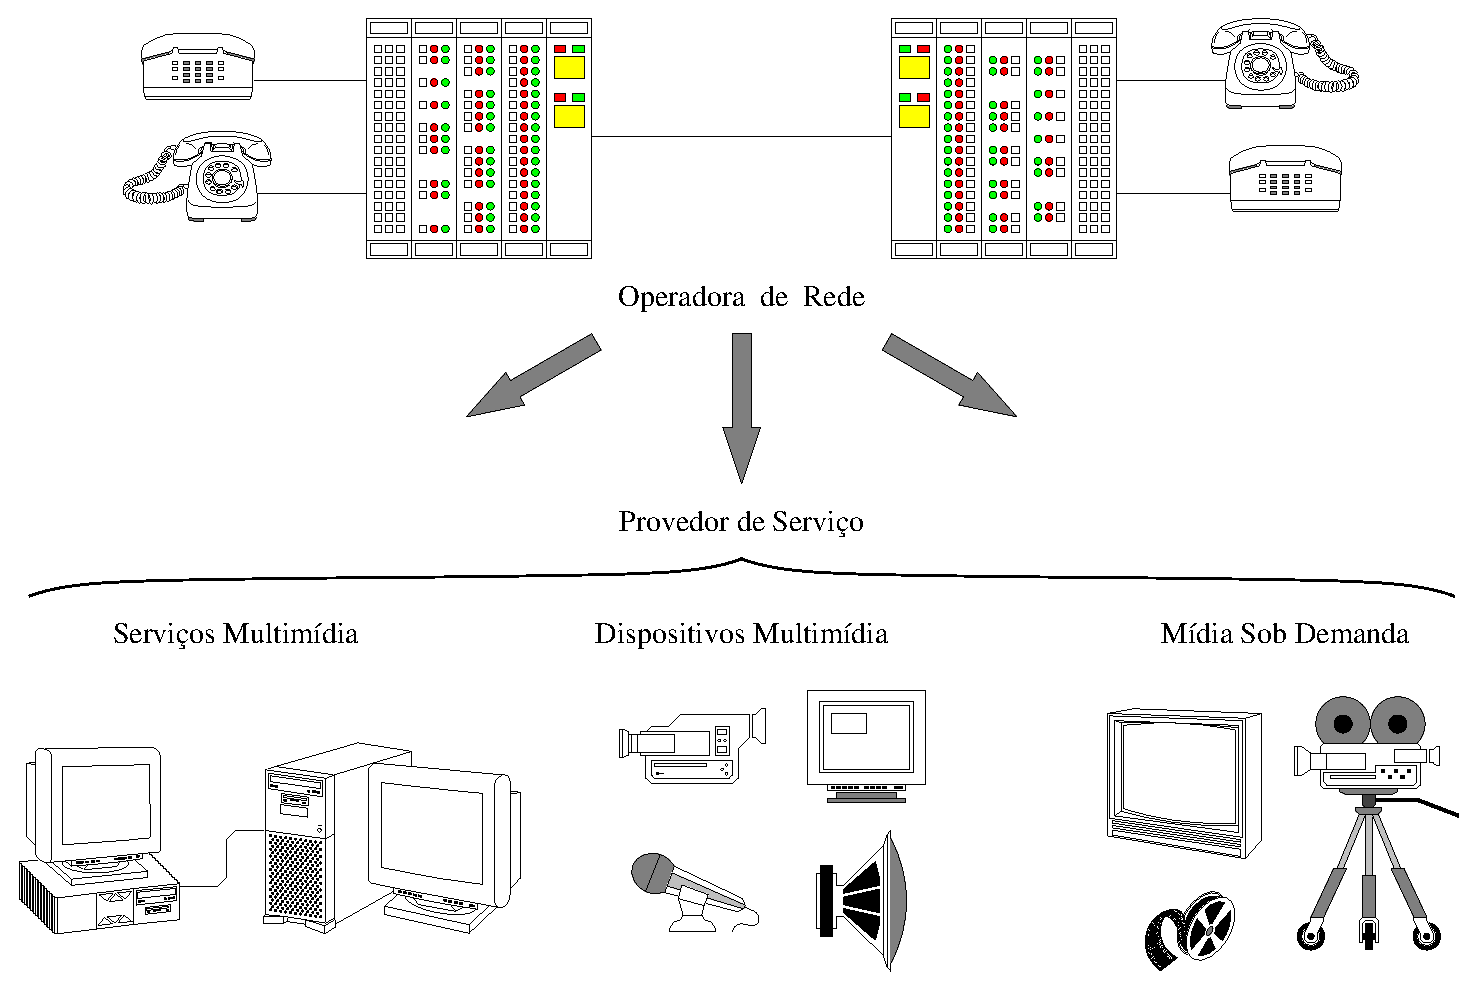
\includegraphics[width=0.55\textwidth]{./CapituloExemplo/figura1}%% Dimens\~oes e localiza\c{c}\~ao
\fonte{\citet{Larsson2003}.}%% Fonte
\end{figure}

Figuras em formato GIF, JPEG e BMP podem ser convertidas para o formato \gls{eps} atrav\'es do aplicativo ``xv''. O ``xv'' n\~ao lista o formato \gls{eps} dentre aqueles que \'e capaz de manipular. Entretanto, selecionando-se o formato \textit{PostScript} e fornecendo-se a extens\~ao \texttt{eps} ao nome do arquivo, o formato \gls{eps} \'e gerado.

O ambiente \texttt{picture} permite a programa\c{c}\~ao de imagens diretamente no \gls{latex}\index{LaTeX@\latex}, conforme exemplo apresentado na \autoref{fig:figura2}.

\begin{figure}[Htb]%% Ambiente figure
\captionsetup{width=8cm}%% Largura da legenda
\caption{Exemplo de figura criada a partir do ambiente \texttt{picture}.}%% Legenda
\label{fig:figura2}%% R\'otulo
\setlength{\unitlength}{1cm}%% Unidade de comprimento
\begin{picture}(8,5)(-4,-2.5)%% Ambiente picture
\put(-4,0){\vector(1,0){8}}
\put(3.75,-0.25){$\chi$}
\put(0,-2.5){\vector(0,1){5}}
\multiput(-4,1)(0.4,0){20}{\line(1,0){0.2}}
\multiput(-4,-1)(0.4,0){20}{\line(1,0){0.2}}
\put(0.25,2.25){$\beta \equiv v / c = \tanh \chi$}
\qbezier(0,0)(0.8853,0.8853)(2,0.9640)
\qbezier(0,0)(-0.8853,-0.8853)(-2,-0.9640)
\end{picture}
\fonte{Autoria pr\'opria.}%% Fonte
\end{figure}

A \autoref{fig:subfigure} apresenta um exemplo usando o pacote \texttt{subfigure} com legendas usando o pacote \texttt{subcaption}. \'E  poss\'{\i}vel referenciar cada uma das sub-figuras, no qual, a sua refer\^encia alfab\'etica aparece entre par\^enteses: \autoref{fig:subfigure_a} e \autoref{fig:subfigure_b}.

\begin{figure}[!ht]
\centering
\caption{Exemplo de Subfigure} 
\label{fig:subfigure}
\begin{subfigure}[t]{.45\textwidth}
	\centering
	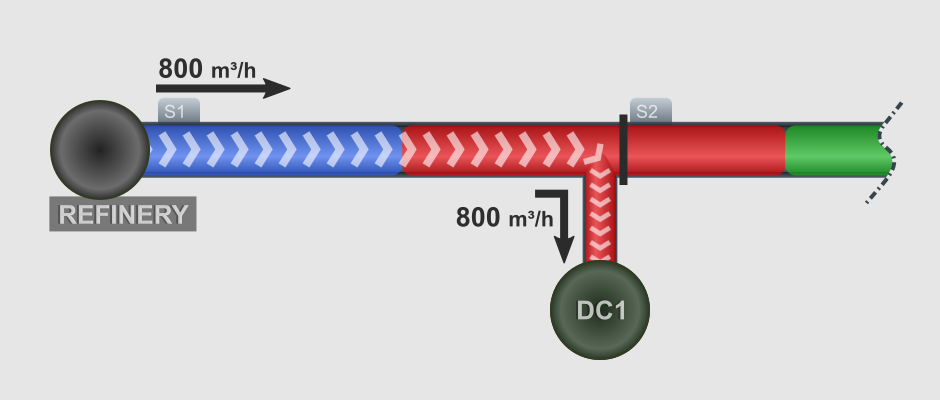
\includegraphics[width=\textwidth]{./CapituloExemplo/subfigure-a.png}
	\caption{Figura A}
	\label{fig:subfigure_a}
\end{subfigure}
\qquad
\begin{subfigure}[t]{.45\textwidth}
	\centering
	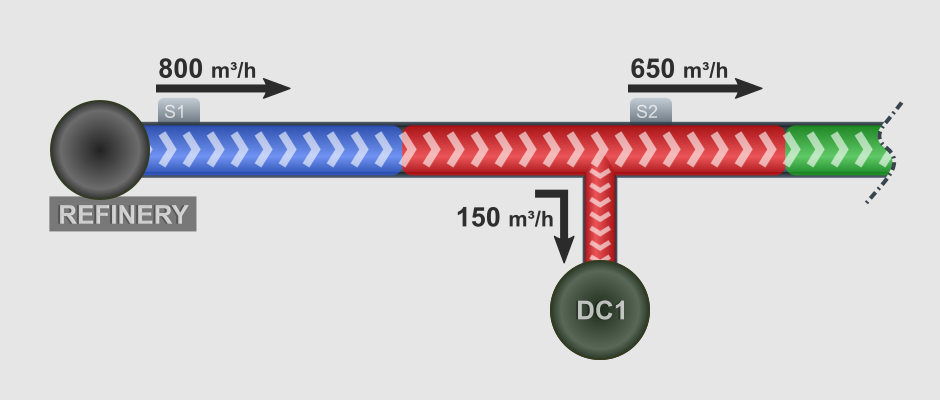
\includegraphics[width=\textwidth]{./CapituloExemplo/subfigure-b.png}  
	\caption{Figura B}
	\label{fig:subfigure_b}
\end{subfigure}
\fonte{\citet{Meira2020}} %citeonline{meira2020}
\end{figure}

%% T\'{\i}tulo e r\'otulo de se\c{c}\~ao (r\'otulos n\~ao devem conter caracteres especiais, acentuados ou cedilha)
\subsection{Fotografias}\label{sec:fotografias}

Um exemplo deste tipo de ilustra\c{c}\~ao \'e apresentado na \autoref{foto:foto1}.

\begin{photograph}[Htb]%% Ambiente photograph
\captionsetup{width=0.6\textwidth}%% Largura da legenda
\caption{Camale\~ao pantera fotografado por Joel Sartore, National Geographic.}%% Legenda
\label{foto:foto1}%% R\'otulo
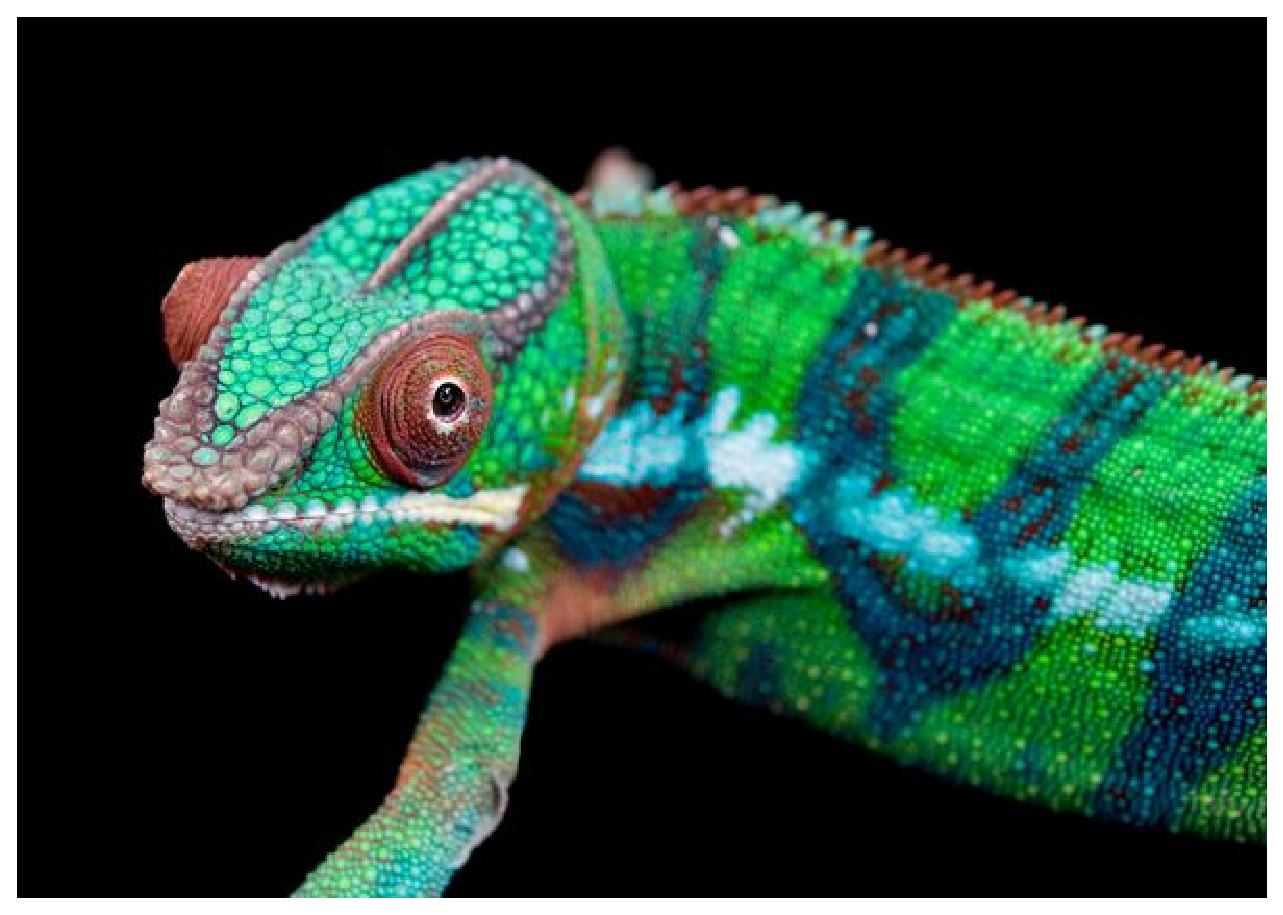
\includegraphics[width=0.6\textwidth]{./CapituloExemplo/foto1}%% Dimens\~oes e localiza\c{c}\~ao
\fonte{\citet{Sartore2013}.}%% Fonte
\end{photograph}

Outro exemplo deste tipo de ilustra\c{c}\~ao \'e apresentado na \autoref{foto:foto2}.

\begin{photograph}[Htb]%% Ambiente photograph
\captionsetup{width=0.6\textwidth}%% Largura da legenda
\caption{Fotografia da erup\c{c}\~ao vulc\^anica em 1982 do Galungung, Indon\'esia (com descargas de raios), produzida pelo Servi\c{c}o Geol\'ogico dos Estados Unidos da Am\'erica.}%% Legenda
\label{foto:foto2}%% R\'otulo
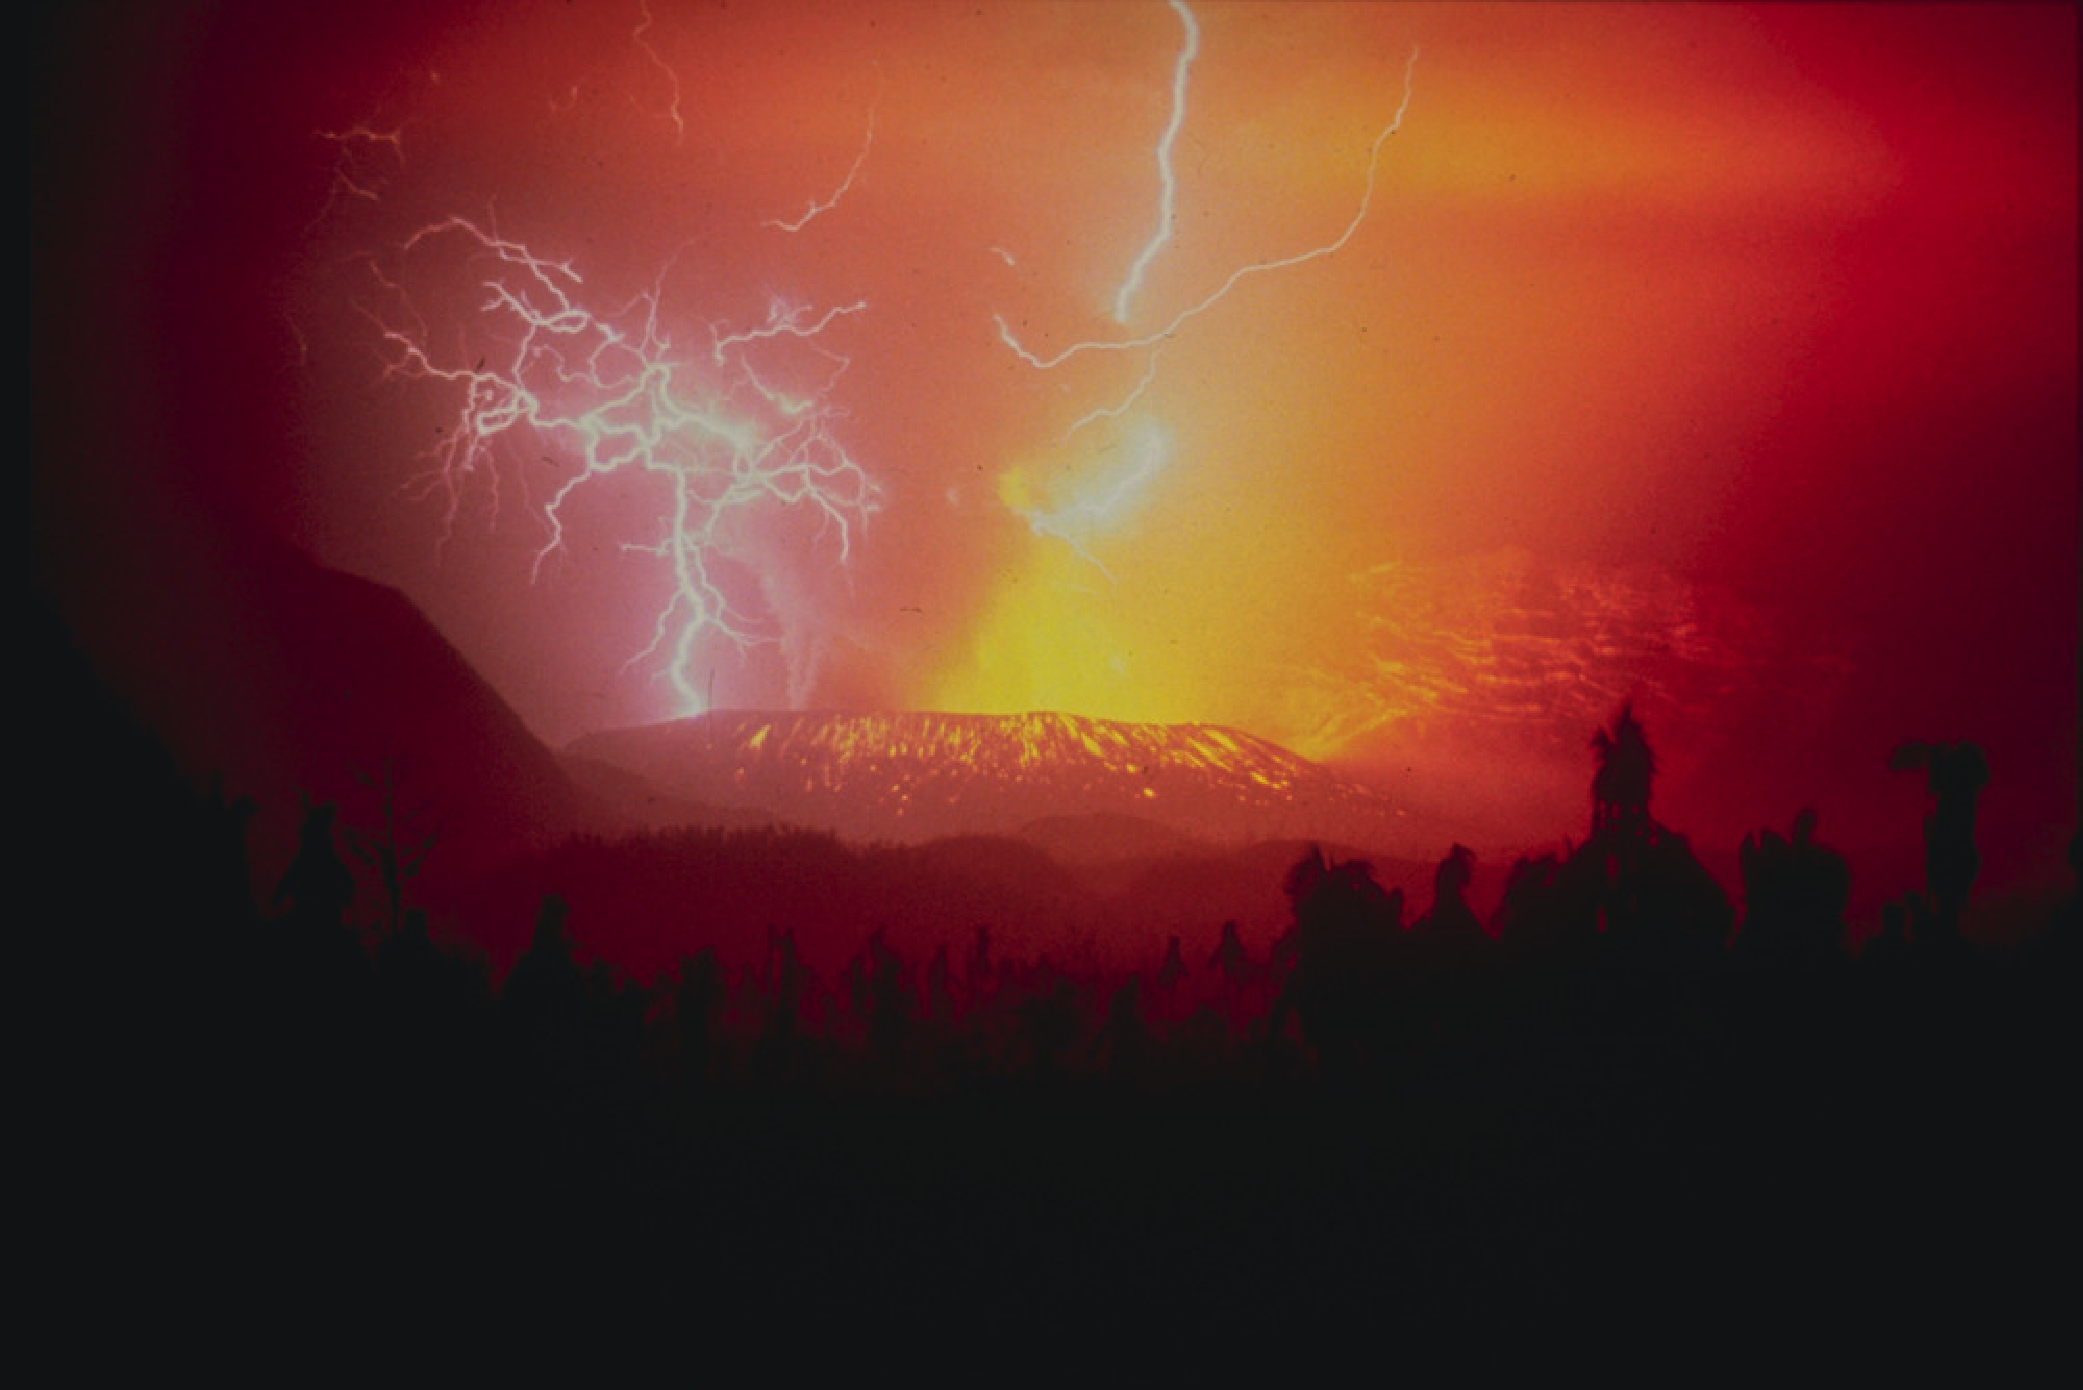
\includegraphics[width=0.6\textwidth]{./CapituloExemplo/foto2}%% Dimens\~oes e localiza\c{c}\~ao
\fonte{\citet{Hadian1982}.}%% Fonte
\end{photograph}

%% T\'{\i}tulo e r\'otulo de se\c{c}\~ao (r\'otulos n\~ao devem conter caracteres especiais, acentuados ou cedilha)
\subsection{Gr\'aficos}\label{sec:graficos}

Gr\'aficos s\~ao gerados com aplicativos capazes de exportar nos formatos \gls{ps} ou \gls{eps}. A ferramenta ``gnuplot'' \'e uma das mais utilizadas para a gera\c{c}\~ao de gr\'aficos (\url{http://www.gnuplot.info/}). Uma vez no formato \gls{eps}, gr\'aficos s\~ao inseridos no texto tal como figuras (veja \autoref{gra:grafico1}).

\begin{graph}[Htb]%% Ambiente graph
\captionsetup{width=0.6\textwidth}%% Largura da legenda
\caption{Exemplo de gr\'afico produzido em ``gnuplot''.}%% Legenda
\label{gra:grafico1}%% R\'otulo
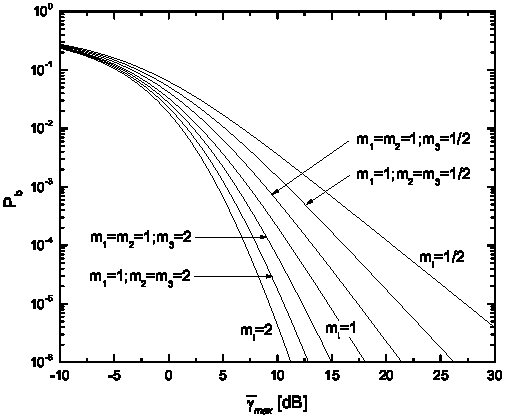
\includegraphics[width=0.6\textwidth]{./CapituloExemplo/grafico1}%% Dimens\~oes e localiza\c{c}\~ao
\fonte{\citet{Faina2001}.}%% Fonte
\end{graph}

No \autoref{gra:grafico2} \'e apresentado um exemplo de gr\'afico produzido em ``Excel''.

\begin{graph}[Htb]%% Ambiente graph
\captionsetup{width=0.6\textwidth}%% Largura da legenda
\caption{Exemplo de gr\'afico produzido em ``Excel''.}%% Legenda
\label{gra:grafico2}%% R\'otulo
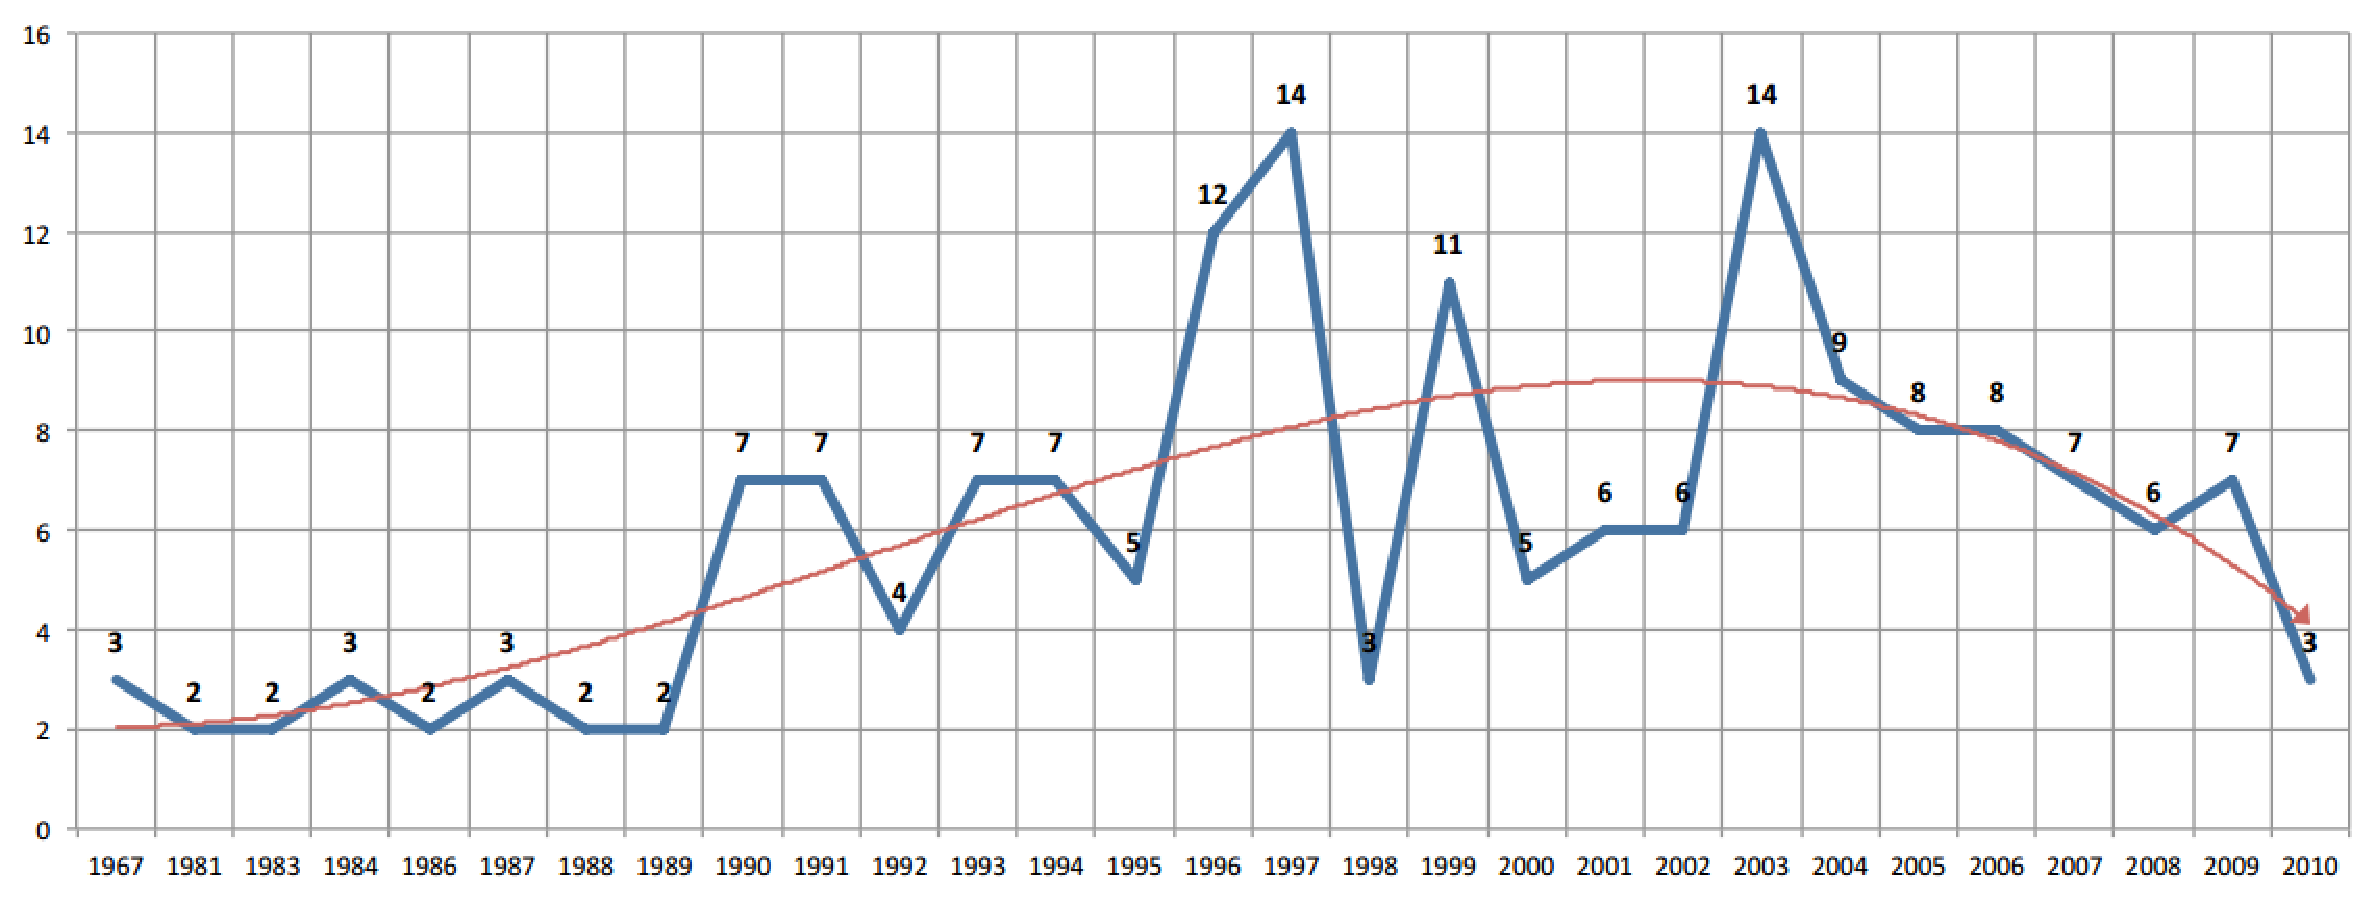
\includegraphics[width=0.6\textwidth]{./CapituloExemplo/grafico2}%% Dimens\~oes e localiza\c{c}\~ao
\fonte{\citeonline[p. 24]{Araujo2012}.}%% Fonte
\end{graph}

O ambiente \texttt{minipage} pode ser usado para inserir textos ou outros elementos em quadros com tamanhos e posi\c{c}\~oes controladas, conforme exemplos apresentados no \autoref{gra:minipagegrafico1} e no \autoref{gra:minipagegrafico2}.

\begin{graph}[Htb]%% Ambiente graph
\begin{minipage}[t]{0.395\textwidth}%% Ambiente minipage
\centering%% Centralizado
\captionsetup{width=0.85\textwidth}%% Largura da legenda
\caption{Gr\'afico 1 do ambiente \texttt{minipage}.}%% Legenda
\label{gra:minipagegrafico1}%% R\'otulo
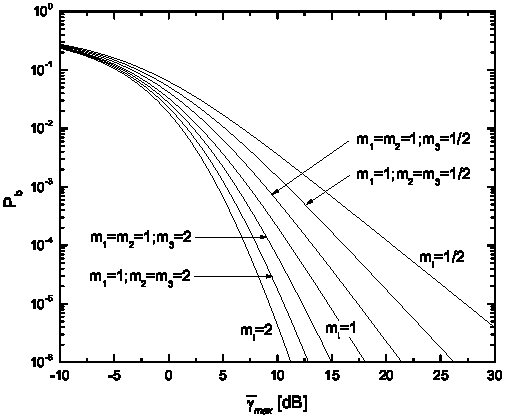
\includegraphics[width=0.85\textwidth]{./CapituloExemplo/grafico1}%% Dimens\~oes e localiza\c{c}\~ao
\fonte{\citet{Faina2001}.}%% Fonte
\end{minipage}
\hfill
\begin{minipage}[t]{0.595\textwidth}%% Ambiente minipage
\centering%% Centralizado
\captionsetup{width=0.95\textwidth}%% Largura da legenda
\caption{Gr\'afico 2 do ambiente \texttt{minipage}.}%% Legenda
\label{gra:minipagegrafico2}%% R\'otulo
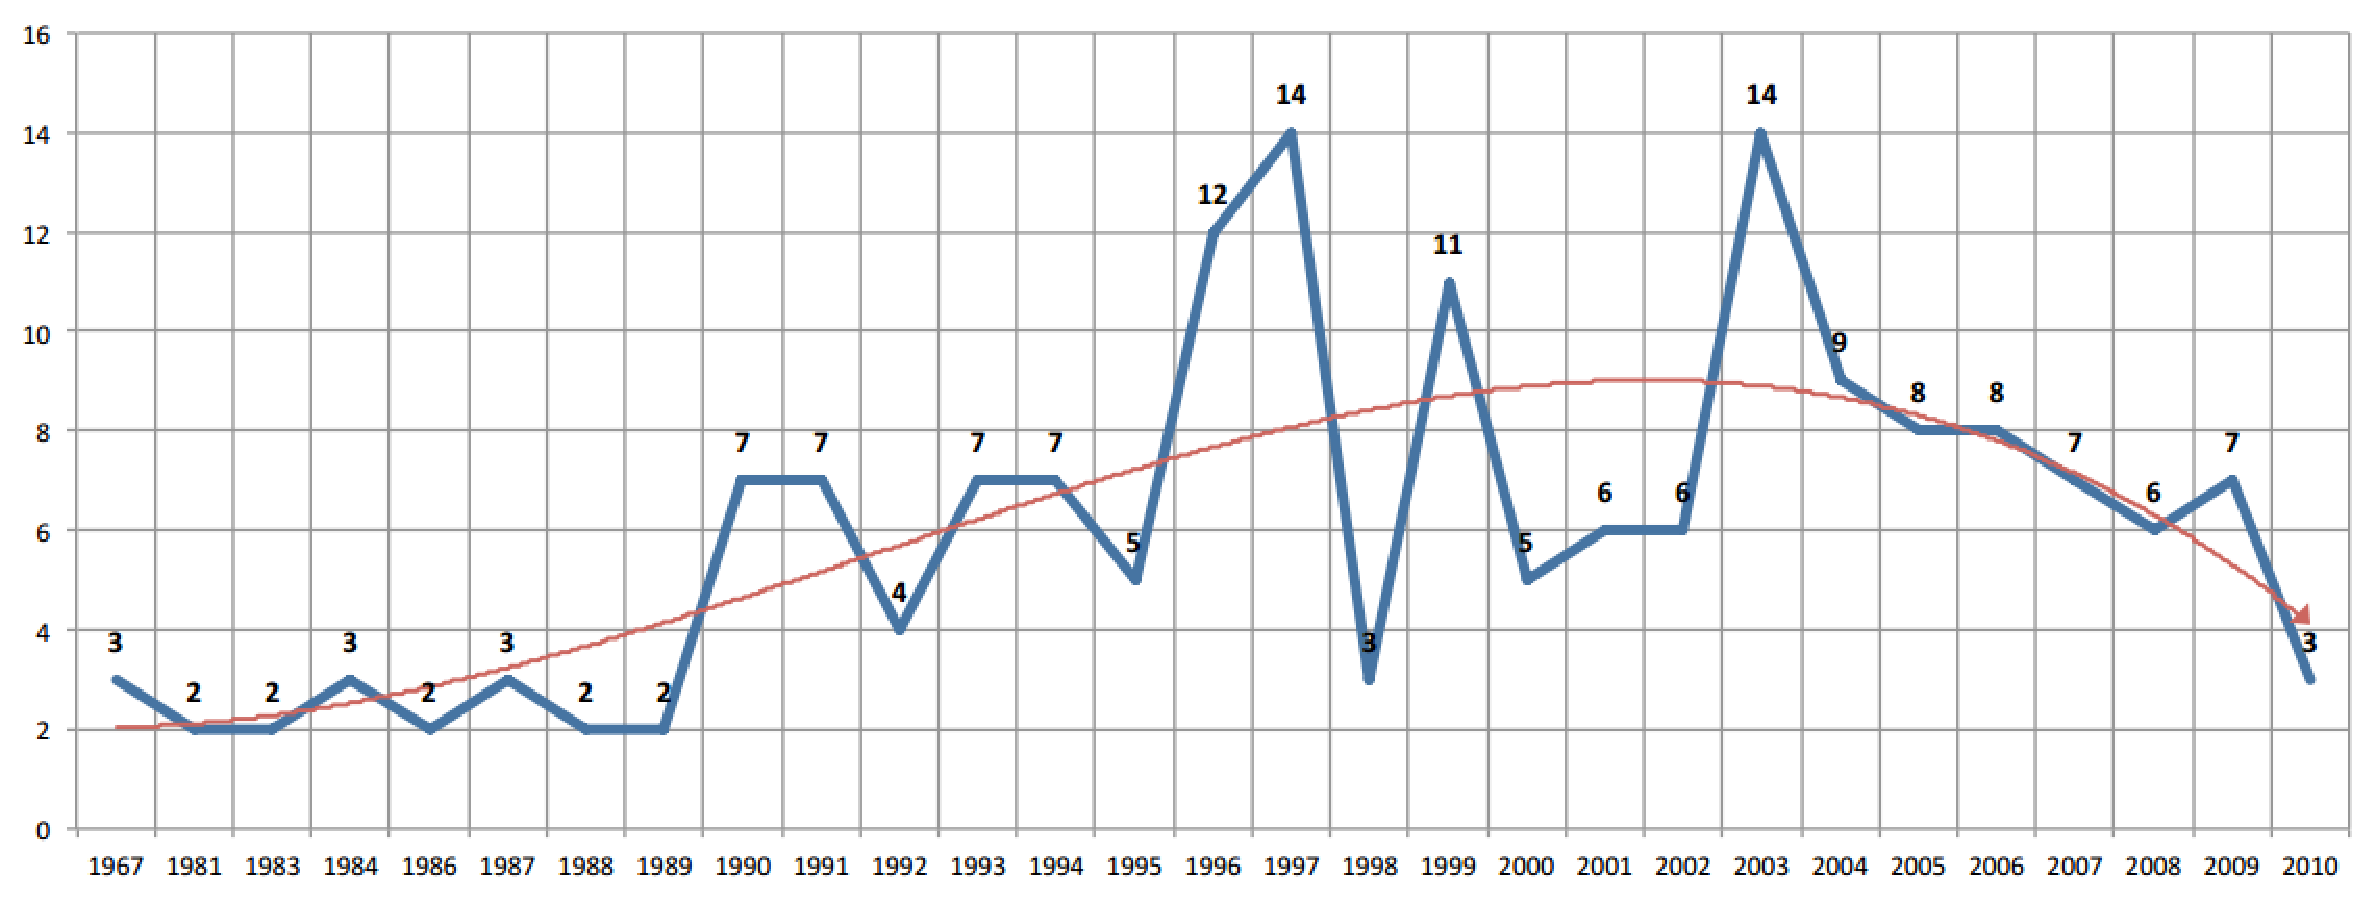
\includegraphics[width=0.95\textwidth]{./CapituloExemplo/grafico2}%% Dimens\~oes e localiza\c{c}\~ao
\fonte{\citeonline[p. 24]{Araujo2012}}%% Fonte
\end{minipage}
\label{gra:minipagegraficos}
\end{graph}

%% T\'{\i}tulo e r\'otulo de se\c{c}\~ao (r\'otulos n\~ao devem conter caracteres especiais, acentuados ou cedilha)
\subsection{Quadros}\label{sec:quadros}

Um exemplo deste tipo de ilustra\c{c}\~ao \'e apresentado no \autoref{quad:quadro1}.

\begin{tabframed}[Htb]%% Ambiente tabframed
\captionsetup{width=0.5\textwidth}%% Largura da legenda
\caption{Compostos org\^anicos: f\'ormulas estruturais e principais classes.}%% Legenda
\label{quad:quadro1}%% R\'otulo
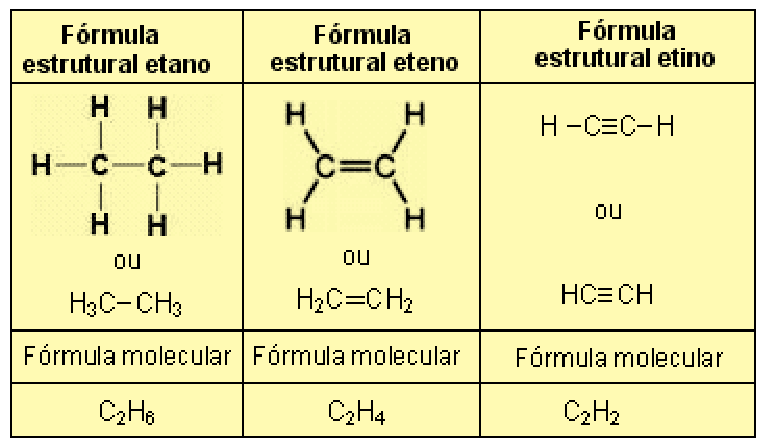
\includegraphics[width=0.5\textwidth]{./CapituloExemplo/quadro1}%% Dimens\~oes e localiza\c{c}\~ao
\fonte{\citet{daSilva2009}.}%% Fonte
\end{tabframed}

Outro exemplo deste tipo de ilustra\c{c}\~ao \'e apresentado no \autoref{quad:quadro2}.

\begin{tabframed}[Htb]%% Ambiente tabframed
\captionsetup{width=0.7\textwidth}%% Largura da legenda
\caption{Modelos de maturidade para a gest\~ao da cadeia de suprimentos.}%% Legenda
\label{quad:quadro2}%% R\'otulo
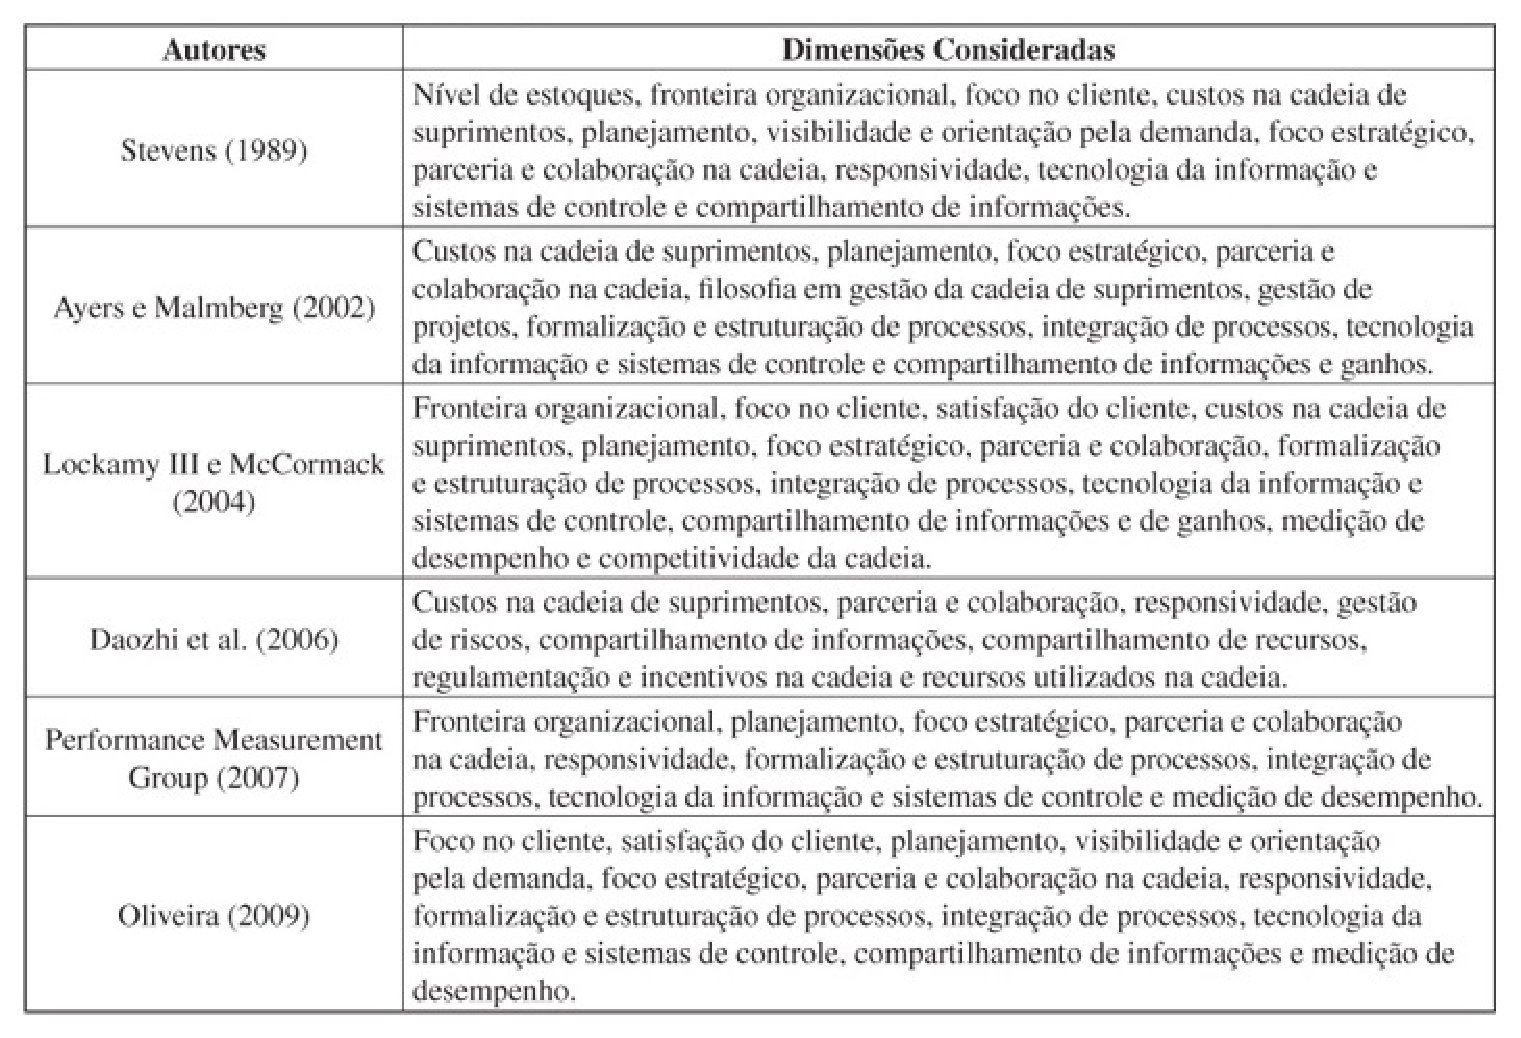
\includegraphics[width=0.7\textwidth]{./CapituloExemplo/quadro2}%% Dimens\~oes e localiza\c{c}\~ao
\fonte{\citet{Frederico2012}.}%% Fonte
\end{tabframed}

Os quadros n\~ao devem ser chamados de tabelas, uma vez que se diferenciam destas por apresentarem as laterais fechadas e o conte\'udo n\~ao num\'erico.

%% T\'{\i}tulo e r\'otulo de se\c{c}\~ao (r\'otulos n\~ao devem conter caracteres especiais, acentuados ou cedilha)
\section{Tabelas}\label{sec:tabelas}

Tabelas s\~ao constru\'{\i}das com comandos pr\'oprios do \gls{latex}\index{LaTeX@\latex}. Por exemplo, a \autoref{tab:tabela1} foi constru\'{\i}da desta forma.

\begin{table}[Htb]%% Ambiente table
\caption{Primeiro exemplo de tabela com uma legenda contendo um texto muito longo que pode ocupar mais de uma linha.}%% Legenda
\label{tab:tabela1}%% R\'otulo
\begin{tabularx}{\textwidth}{@{\extracolsep{\fill}}llll}%% Ambiente tabularx
\toprule
$\bsym{L}$ & $\bsym{L^2}$ & $\bsym{L^3}$ & $\bsym{L^4}$ \\
\SI{}{[m]} & \SI{}{[m^2]} & \SI{}{[m^3]} & \SI{}{[m^4]} \\ \midrule
1          & 1            & 1            & 1            \\
2          & 4            & 8            & 16           \\
3          & 9            & 27           & 81           \\
4          & 16           & 64           & 256          \\
5          & 25           & 125          & 625          \\ \bottomrule
\end{tabularx}
\fonte{Autoria pr\'opria.}%% Fonte
\end{table}

A \autoref{tab:tabela2} \'e um exemplo de tabela que ocupa mais de uma p\'agina e que foi constru\'{\i}da pelo \gls{latex}\index{LaTeX@\latex} utilizando o pacote \texttt{longtable}.

\begin{longtable}{@{\extracolsep{\fill}}lll}%% Ambiente longtable
\caption{Poss\'{\i}veis tr\'{\i}plices para grade altamente vari\'avel.\label{tab:tabela2}} \\%% Legenda e r\'otulo
\toprule
\textbf{Tempo (s)} & \textbf{Tr\'{\i}plice escolhida} & \textbf{Outras poss\'{\i}veis tr\'{\i}plices} \\
\midrule
\endfirsthead%% Encerra cabe\c{c}alho da primeira p\'agina
\caption[]{Poss\'{\i}veis tr\'{\i}plices para grade altamente vari\'avel.} \\%% Legenda
\multicolumn{3}{r}{\textbf{(continua\c{c}\~ao)}} \\
\toprule
\textbf{Tempo (s)} & \textbf{Tr\'{\i}plice escolhida} & \textbf{Outras poss\'{\i}veis tr\'{\i}plices} \\
\midrule
\endhead%% Encerra cabe\c{c}alho das demais p\'aginas
\midrule
\multicolumn{3}{r}{\textbf{(continua)}} \\
\endfoot%% Encerra rodap\'e das demais p\'aginas
\bottomrule
\\[-0.5\linha]
\caption*{\nomefonte: Adaptado de \citet{Smallen2014}.} \\
\endlastfoot%% Encerra rodap\'e da \'ultima p\'agina
0      & (1, 11, 13725) & (1, 12, 10980), (1, 13, 8235), (2, 2, 0), (3, 1, 0) \\
2745   & (1, 12, 10980) & (1, 13, 8235), (2, 2, 0), (2, 3, 0), (3, 1, 0)      \\
5490   & (1, 12, 13725) & (2, 2, 2745), (2, 3, 0), (3, 1, 0)                  \\
8235   & (1, 12, 16470) & (1, 13, 13725), (2, 2, 2745), (2, 3, 0), (3, 1, 0)  \\
10980  & (1, 12, 16470) & (1, 13, 13725), (2, 2, 2745), (2, 3, 0), (3, 1, 0)  \\
13725  & (1, 12, 16470) & (1, 13, 13725), (2, 2, 2745), (2, 3, 0), (3, 1, 0)  \\
16470  & (1, 13, 16470) & (2, 2, 2745), (2, 3, 0), (3, 1, 0)                  \\
19215  & (1, 12, 16470) & (1, 13, 13725), (2, 2, 2745), (2, 3, 0), (3, 1, 0)  \\
21960  & (1, 12, 16470) & (1, 13, 13725), (2, 2, 2745), (2, 3, 0), (3, 1, 0)  \\
24705  & (1, 12, 16470) & (1, 13, 13725), (2, 2, 2745), (2, 3, 0), (3, 1, 0)  \\
27450  & (1, 12, 16470) & (1, 13, 13725), (2, 2, 2745), (2, 3, 0), (3, 1, 0)  \\
30195  & (2, 2, 2745)   & (2, 3, 0), (3, 1, 0)                                \\
32940  & (1, 13, 16470) & (2, 2, 2745), (2, 3, 0), (3, 1, 0)                  \\
35685  & (1, 13, 13725) & (2, 2, 2745), (2, 3, 0), (3, 1, 0)                  \\
38430  & (1, 13, 10980) & (2, 2, 2745), (2, 3, 0), (3, 1, 0)                  \\
41175  & (1, 12, 13725) & (1, 13, 10980), (2, 2, 2745), (2, 3, 0), (3, 1, 0)  \\
43920  & (1, 13, 10980) & (2, 2, 2745), (2, 3, 0), (3, 1, 0)                  \\
46665  & (2, 2, 2745)   & (2, 3, 0), (3, 1, 0)                                \\
49410  & (2, 2, 2745)   & (2, 3, 0), (3, 1, 0)                                \\
52155  & (1, 12, 16470) & (1, 13, 13725), (2, 2, 2745), (2, 3, 0), (3, 1, 0)  \\
54900  & (1, 13, 13725) & (2, 2, 2745), (2, 3, 0), (3, 1, 0)                  \\
57645  & (1, 13, 13725) & (2, 2, 2745), (2, 3, 0), (3, 1, 0)                  \\
60390  & (1, 12, 13725) & (2, 2, 2745), (2, 3, 0), (3, 1, 0)                  \\
63135  & (1, 13, 16470) & (2, 2, 2745), (2, 3, 0), (3, 1, 0)                  \\
65880  & (1, 13, 16470) & (2, 2, 2745), (2, 3, 0), (3, 1, 0)                  \\
68625  & (2, 2, 2745)   & (2, 3, 0), (3, 1, 0)                                \\
71370  & (1, 13, 13725) & (2, 2, 2745), (2, 3, 0), (3, 1, 0)                  \\
74115  & (1, 12, 13725) & (2, 2, 2745), (2, 3, 0), (3, 1, 0)                  \\
76860  & (1, 13, 13725) & (2, 2, 2745), (2, 3, 0), (3, 1, 0)                  \\
79605  & (1, 13, 13725) & (2, 2, 2745), (2, 3, 0), (3, 1, 0)                  \\
82350  & (1, 12, 13725) & (2, 2, 2745), (2, 3, 0), (3, 1, 0)                  \\
85095  & (1, 12, 13725) & (1, 13, 10980), (2, 2, 2745), (2, 3, 0), (3, 1, 0)  \\
87840  & (1, 13, 16470) & (2, 2, 2745), (2, 3, 0), (3, 1, 0)                  \\
90585  & (1, 13, 16470) & (2, 2, 2745), (2, 3, 0), (3, 1, 0)                  \\
93330  & (1, 13, 13725) & (2, 2, 2745), (2, 3, 0), (3, 1, 0)                  \\
96075  & (1, 13, 16470) & (2, 2, 2745), (2, 3, 0), (3, 1, 0)                  \\
98820  & (1, 13, 16470) & (2, 2, 2745), (2, 3, 0), (3, 1, 0)                  \\
101565 & (1, 13, 13725) & (2, 2, 2745), (2, 3, 0), (3, 1, 0)                  \\
104310 & (1, 13, 16470) & (2, 2, 2745), (2, 3, 0), (3, 1, 0)                  \\
107055 & (1, 13, 13725) & (2, 2, 2745), (2, 3, 0), (3, 1, 0)                  \\
109800 & (1, 13, 13725) & (2, 2, 2745), (2, 3, 0), (3, 1, 0)                  \\
112545 & (1, 12, 16470) & (1, 13, 13725), (2, 2, 2745), (2, 3, 0), (3, 1, 0)  \\
115290 & (1, 13, 16470) & (2, 2, 2745), (2, 3, 0), (3, 1, 0)                  \\
118035 & (1, 13, 13725) & (2, 2, 2745), (2, 3, 0), (3, 1, 0)                  \\
120780 & (1, 13, 16470) & (2, 2, 2745), (2, 3, 0), (3, 1, 0)                  \\
123525 & (1, 13, 13725) & (2, 2, 2745), (2, 3, 0), (3, 1, 0)                  \\
126270 & (1, 12, 16470) & (1, 13, 13725), (2, 2, 2745), (2, 3, 0), (3, 1, 0)  \\
129015 & (2, 2, 2745)   & (2, 3, 0), (3, 1, 0)                                \\
131760 & (2, 2, 2745)   & (2, 3, 0), (3, 1, 0)                                \\
134505 & (1, 13, 16470) & (2, 2, 2745), (2, 3, 0), (3, 1, 0)                  \\
137250 & (1, 13, 13725) & (2, 2, 2745), (2, 3, 0), (3, 1, 0)                  \\
139995 & (2, 2, 2745)   & (2, 3, 0), (3, 1, 0)                                \\
142740 & (2, 2, 2745)   & (2, 3, 0), (3, 1, 0)                                \\
145485 & (1, 12, 16470) & (1, 13, 13725), (2, 2, 2745), (2, 3, 0), (3, 1, 0)  \\
148230 & (2, 2, 2745)   & (2, 3, 0), (3, 1, 0)                                \\
150975 & (1, 13, 16470) & (2, 2, 2745), (2, 3, 0), (3, 1, 0)                  \\
153720 & (1, 12, 13725) & (2, 2, 2745), (2, 3, 0), (3, 1, 0)                  \\
156465 & (1, 13, 13725) & (2, 2, 2745), (2, 3, 0), (3, 1, 0)                  \\
159210 & (1, 13, 13725) & (2, 2, 2745), (2, 3, 0), (3, 1, 0)                  \\
161955 & (1, 13, 16470) & (2, 2, 2745), (2, 3, 0), (3, 1, 0)                  \\
164700 & (1, 13, 13725) & (2, 2, 2745), (2, 3, 0), (3, 1, 0)                  \\
\end{longtable}

Tabelas criadas em planilhas do ``Excel'' podem ser convertidas em tabelas \gls{latex}\index{LaTeX@\latex} atrav\'es do suplemento ``Excel-to-LaTeX'', dispon\'{\i}vel em \url{http://www.ctan.org/pkg/excel2latex}.

%% T\'{\i}tulo e r\'otulo de se\c{c}\~ao (r\'otulos n\~ao devem conter caracteres especiais, acentuados ou cedilha)
\section{Abreviaturas, Siglas e Acr\^onimos}\label{sec:acronimos}

\gls{latex}\index{LaTeX@\latex} gera automaticamente a lista de abreviaturas, siglas e acr\^onimos atrav\'es do pacote \texttt{glossaries}. As abreviaturas, siglas e acr\^onimos devem ser definidos no arquivo \texttt{entradas-acronimos.tex}, no diret\'orio ``PreTexto'', com os comandos:

\begin{SingleSpacing}%% Ambiente SingleSpacing
\begin{verbatim}
\abreviatura{r\'otulo}{representa\c{c}\~ao}{defini\c{c}\~ao}
\sigla{r\'otulo}{representa\c{c}\~ao}{defini\c{c}\~ao}
\acronimo{r\'otulo}{representa\c{c}\~ao}{defini\c{c}\~ao}
\end{verbatim}
\end{SingleSpacing}

Para que a abreviatura, sigla ou acr\^onimo seja apresentada em alguma parte do texto do documento use o comando \verb|\gls{r\'otulo}|, por exemplo, as abreviaturas \gls{art.}, \gls{cap.} e \gls{sec.} foram geradas pelos comandos \verb|\gls{art.}, \gls{cap.} e \gls{sec.}|, respectivamente. Mais detalhes dos comandos do pacote \texttt{glossaries} podem ser encontrados em: \url{http://mirrors.ctan.org/macros/latex/contrib/glossaries/glossaries-user.pdf}.

Outra op\c{c}\~ao para gerar a lista de abreviaturas, siglas e acr\^onimos \'e atrav\'es da edi\c{c}\~ao manual do arquivo \texttt{lista-acronimos.tex} no diret\'orio ``PreTexto''.

%% T\'{\i}tulo e r\'otulo de se\c{c}\~ao (r\'otulos n\~ao devem conter caracteres especiais, acentuados ou cedilha)
\section{S\'{\i}mbolos}\label{sec:simbolos}

\gls{latex}\index{LaTeX@\latex} gera automaticamente a lista de s\'{\i}mbolos atrav\'es do pacote \texttt{nomencl}. Ao redigir um s\'{\i}mbolo pela primeira vez em qualquer parte do texto com o comando \verb|\nomenclature[prefixo]{s\'{\i}mbolo}{descri\c{c}\~ao \nomunit{unidade}}|, \'e gerada uma entrada para a lista de s\'{\i}mbolos. Veja exemplos deste comando no arquivo fonte deste cap\'{\i}tulo. Os elementos da lista de s\'{\i}mbolos s\~ao ordenados a depender da primeira letra atribu\'{\i}da ao prefixo e classificadas em:

\begin{itemize}%% Lista de itens
\item A~-~Letras Latinas.
\item B~-~Letras Gregas.
\item C~-~Sobrescritos.
\item D~-~Subscritos.
\item E~-~Nota\c{c}\~oes.
\item F~-~\'Indices e Conjuntos
\item G~-~Par\^ametros
\item H~-~Vari\'aveis cont\'{\i}nuas
\item I~-~Vari\'aveis inteiras
\item J~-~Vari\'aveis bin\'arias
\end{itemize}

Outra op\c{c}\~ao ao comando \verb|\nomenclature| \'e o uso dos atalhos:

\begin{SingleSpacing}%% Ambiente SingleSpacing
\begin{verbatim}
\letralatina{prefixo}{s\'{\i}mbolo}{descri\c{c}\~ao}{unidade}
\letragrega{prefixo}{s\'{\i}mbolo}{descri\c{c}\~ao}{unidade}
\sobrescrito{prefixo}{s\'{\i}mbolo}{descri\c{c}\~ao}{unidade}
\subscrito{prefixo}{s\'{\i}mbolo}{descri\c{c}\~ao}{unidade}
\notacao{prefixo}{s\'{\i}mbolo}{descri\c{c}\~ao}{unidade}
\notacaois{s\'{\i}mbolo}{descri\c{c}\~ao}{unidade}
\notacaoparam{s\'{\i}mbolo}{descri\c{c}\~ao}{unidade}
\notacaofloatvar{s\'{\i}mbolo}{descri\c{c}\~ao}{unidade}
\notacaointvar{s\'{\i}mbolo}{descri\c{c}\~ao}{unidade}
\notacaobinvar{s\'{\i}mbolo}{descri\c{c}\~ao}{unidade}
\end{verbatim}
\end{SingleSpacing}

\noindent Neste caso a atribui\c{c}\~ao da primeira letra do prefixo pode ser desprezada.

%% Letras Latinas [A]
\nomenclature[AA]{$A$}{\'Area \nomunit{m^2}}%%
\letralatina{L}{L}{Comprimento}{m}%%
\letralatina{R}{R}{Raio}{m}%%
%% Letras Gregas [B]
\nomenclature[Bmu]{$\mu$}{Viscosidade din\^amica \nomunit{kg/(m.s)}}%%
\letragrega{nu}{\nu}{Viscosidade cinem\'atica}{m^2/s}%%
\letragrega{pi}{\pi}{Pi (constante circular)}{rad}%%
\letragrega{rho}{\rho}{Massa espec\'{\i}fica}{kg/m^3}%%
\letragrega{sigma}{\sigma}{Tens\~ao superficial}{N/m}%%
%% Sobrescritos [C]
\nomenclature[C+]{$+$}{Passo de tempo posterior}%%
\sobrescrito{-}{-}{Passo de tempo anterior}{}%%
\sobrescrito{0}{0}{Valor inicial}{}%%
%% Subscritos [D]
\nomenclature[DG]{$G$}{Fase gasosa}%%
\subscrito{L}{L}{Fase l\'{\i}quida}{}%%
\subscrito{S}{S}{Fase s\'olida}{}%%
%% Nota\c{c}\~oes [E]
\nomenclature[EPsi_1]{$\overline{\Psi}$}{M\'edia temporal}%%
\notacao{Psi_2}{\langle \Psi \rangle}{M\'edia na se\c{c}\~ao transversal}{}%%
\notacao{Psi_3}{\langle\langle \Psi \rangle\rangle}{M\'edia na se\c{c}\~ao transversal ponderada}{}%%
%% Nota\c{c}\~oes [F]
\notacaois{Event_set}{e \in E}{Set of events}{}
\notacaois{Interval_set}{i \in I}{Set of intervals}{}
%% Nota\c{c}\~oes [H]
\notacaoparam{eps}{\varepsilon}{Small constant value}{}
\notacaoparam{lb}{L}{Lower bound value ($L \ll 0$)}{}
%% Nota\c{c}\~oes [I]
\notacaofloatvar{end}{e_{i}}{End of interval $i$}{h}
\notacaofloatvar{start}{s_{i}}{Start of interval $i$}{h}
%% Nota\c{c}\~oes [J]
\notacaointvar{e_i}{\phi_i}{Number of employees set to work during interval $i$}{}
%% Nota\c{c}\~oes [K]
\notacaobinvar{a_i}{a_{i}}{1 if the flow is active during interval $i$; 0 otherwise}{}

Mais detalhes dos comandos do pacote \texttt{nomencl} podem ser encontrados em: \url{http://tug.ctan.org/tex-archive/macros/latex/contrib/nomencl/nomencl.pdf}.

Outra op\c{c}\~ao para gerar a lista de s\'{\i}mbolos \'e atrav\'es da edi\c{c}\~ao manual do arquivo \texttt{lista-simbolos.tex} no diret\'orio ``PreTexto''.

%% T\'{\i}tulo e r\'otulo de se\c{c}\~ao (r\'otulos n\~ao devem conter caracteres especiais, acentuados ou cedilha)
\section{Inclus\~ao de Outros Arquivos}\label{sec:inclusao}

\'E uma boa pr\'atica dividir o seu documento em diversos arquivos, e n\~ao apenas escrever tudo em um \'unico. Esse recurso foi utilizado neste documento (veja \texttt{utfprct.tex}). Para incluir diferentes arquivos em um arquivo principal, de modo que cada arquivo inclu\'{\i}do fique em uma p\'agina diferente, utilize o comando:

\begin{SingleSpacing}%% Ambiente SingleSpacing
\begin{verbatim}
\include{documento-a-ser-incluido} %% Sem a extens\~ao .tex
\end{verbatim}
\end{SingleSpacing}

Para incluir documentos sem quebra de p\'aginas, utilize:

\begin{SingleSpacing}%% Ambiente SingleSpacing
\begin{verbatim}
\input{documento-a-ser-incluido}   %% Sem a extens\~ao .tex
\end{verbatim}
\end{SingleSpacing}

%% T\'{\i}tulo e r\'otulo de se\c{c}\~ao (r\'otulos n\~ao devem conter caracteres especiais, acentuados ou cedilha)
\section{Refer\^encias Bibliogr\'aficas}\label{sec:referencias}

A formata\c{c}\~ao das refer\^encias bibliogr\'aficas conforme as regras da \gls{abnt}\index{ABNT} s\~ao um dos principais objetivos do \gls{abntex2}\index{abnTeX2@\abnTeX}. Consulte os manuais \citeonline{abnTeX2:2013Cite} e \citeonline{abnTeX2:2013CiteAlf} para obter informa\c{c}\~oes sobre sua utiliza\c{c}\~ao.

%% T\'{\i}tulo e r\'otulo de se\c{c}\~ao (r\'otulos n\~ao devem conter caracteres especiais, acentuados ou cedilha)
\subsection{Acentua\c{c}\~ao de Refer\^encias Bibliogr\'aficas}\label{sec:acentuacaodereferencias}

Normalmente n\~ao h\'a problemas em usar caracteres acentuados em arquivos bibliogr\'aficos (extens\~ao \texttt{bib}). Por\'em, como as regras da \gls{abnt}\index{ABNT} fazem uso quase abusivo da convers\~ao para letras mai\'usculas, \'e preciso observar o modo como se escreve os nomes dos autores e/ou editores. No \autoref{quad:quadro3} voc\^e encontra alguns exemplos das convers\~oes mais importantes. A regra geral \'e sempre usar a acentua\c{c}\~ao neste modo quando houver convers\~ao para letras mai\'usculas.

\begin{tabframed}[Htb]%% Ambiente tabframed
\captionsetup{width=0.5\textwidth}%% Largura da legenda
\caption{Convers\~ao de acentua\c{c}\~ao em arquivos \texttt{bibtex}.}%% Legenda
\label{quad:quadro3}%% R\'otulo
\begin{tabular}{|*{2}{p{0.25\textwidth-\columnsep}|}}%% Ambiente tabular
\toprule
\textbf{Acento}   & \textbf{Comando}                       \\ \midrule
{\'a} {\`a} {\~a} & \verb|{\'a}| \verb|{\`a}| \verb|{\~a}| \\ \midrule
{\^e}             & \verb|{\^e}|                           \\ \midrule
{\"u}             & \verb|{\"u}|                           \\ \midrule
{\'\i}            & \verb|{\'\i}|                          \\ \midrule
{\c{c}}           & \verb|{\c{c}}|                         \\ \bottomrule
\end{tabular}
\fonte{Autoria pr\'opria.}%% Fonte
\end{tabframed}

%% T\'{\i}tulo e r\'otulo de se\c{c}\~ao (r\'otulos n\~ao devem conter caracteres especiais, acentuados ou cedilha)
\section{Gloss\'ario}\label{sec:glossario}

Voc\^e pode definir as entradas do gloss\'ario no in\'{\i}cio do texto. Recomenda-se o uso de um arquivo separado a ser inserido ainda no pre\^ambulo do documento, como por exemplo o arquivo \texttt{entradas-glossario.tex} no diret\'orio ``PosTexto'' do presente documento. Veja orienta\c{c}\~oes sobre inclus\~ao de arquivos na \autoref{sec:inclusao}.

`O \gls{abntex2} \'e \glsdesc*{abntex2}' \'e um exemplo de termo definido no gloss\'ario e usado no decorrer do texto, bem como:

\begin{citacao}%% Ambiente citacao
Esta frase usa a palavra \gls{componente} e o plural de \glspl{filho}, ambas definidas no gloss\'ario como filhas da entrada \gls{pai}. \Gls{equilibrio} exemplifica o uso de um termo no in\'{\i}cio da frase. O software \gls{abntex2}\index{abnTeX2@\abnTeX} \'e escrito em \gls{latex}\index{LaTeX@\latex}, que \'e definido no gloss\'ario como `\glsdesc*{latex}'.
\end{citacao}

A frase da cita\c{c}\~ao direta acima foi produzida com:

\begin{SingleSpacing}%% Ambiente SingleSpacing
\begin{verbatim}
Esta frase usa a palavra \gls{componente} e o plural de
\glspl{filho}, ambas definidas no gloss\'ario como filhas da
entrada \gls{pai}. \Gls{equilibrio} exemplifica o uso de um
termo no in\'{\i}cio da frase. O software \gls{abntex2} \'e
escrito em \gls{latex}, que \'e definido no gloss\'ario como
`\glsdesc*{latex}'.
\end{verbatim}
\end{SingleSpacing}

A impress\~ao efetiva do gloss\'ario \'e dada com:

\begin{SingleSpacing}%% Ambiente SingleSpacing
\begin{verbatim}
\printglossaries
\end{verbatim}
\end{SingleSpacing}

A impress\~ao do gloss\'ario incorpora o n\'umero das p\'aginas em que as entradas foram citadas. Isso pode ser removido adicionando-se a op\c{c}\~ao \texttt{nonumberlist} em:

\begin{SingleSpacing}%% Ambiente SingleSpacing
\begin{verbatim}
\usepackage[nonumberlist, style=index]{glossaries}
\end{verbatim}
\end{SingleSpacing}

%% T\'{\i}tulo e r\'otulo de se\c{c}\~ao (r\'otulos n\~ao devem conter caracteres especiais, acentuados ou cedilha)
\section{Ap\^endices e Anexos}\label{sec:apendiceseanexos}

Ap\^endices e anexos podem ser inseridos no documento, logo ap\'os o gloss\'ario, atrav\'es da inclus\~ao de arquivos, como por exemplo, os arquivos fontes \texttt{apendicea.tex}, \texttt{apendiceb.tex} e  \texttt{anexoa.tex}, presentes no diret\'orio ``PosTexto'' deste projeto, s\~ao utilizados para gerar o \autoref{cap:apendicea}, o \autoref{cap:apendiceb} e o \autoref{cap:anexoa}, respectivamente. Veja orienta\c{c}\~oes sobre inclus\~ao de arquivos na \autoref{sec:inclusao}.

%% T\'{\i}tulo e r\'otulo de se\c{c}\~ao (r\'otulos n\~ao devem conter caracteres especiais, acentuados ou cedilha)
\section{\'Indice Remissivo}\label{sec:indice}

Palavras podem ser indexadas no \'{\i}ndice remissivo atrav\'es do comando \verb|\index{palavra a ser indexada}|. Existem v\'arios exemplos do uso deste comando no arquivo fonte deste cap\'{\i}tulo. Por exemplo o comando \verb|\index{Windows}| \'e utilizado para indexar a palavra Windows\index{Windows} no \'{\i}ndice remissivo.

%% T\'{\i}tulo e r\'otulo de se\c{c}\~ao (r\'otulos n\~ao devem conter caracteres especiais, acentuados ou cedilha)
\section{Compila\c{c}\~ao do Documento \LaTeX}\label{sec:compilar}\index{LaTeX@\latex}

Geralmente os editores \gls{latex}\index{LaTeX@\latex}, como o TeXlipse\index{TeXlipse}\footnote{Dispon\'{\i}vel em \url{http://texlipse.sourceforge.net/}.}, o Texmaker\index{Texmaker}\footnote{Dispon\'{\i}vel em \url{http://www.xm1math.net/texmaker/}.}, entre outros, compilam os documentos automaticamente ou ap\'os configura\c{c}\~ao, de modo que voc\^e n\~ao precisa se preocupar com isto.

No entanto, voc\^e pode compilar os documentos \gls{latex}\index{LaTeX@\latex} usando os seguintes comandos, que devem ser digitados no \textit{Prompt} de comandos do Windows\index{Windows} ou no terminal do Mac\index{Mac} ou do Linux\index{Linux}:

\begin{SingleSpacing}%% Ambiente SingleSpacing
\begin{verbatim}
latex <mainfile>.tex
bibtex <mainfile>
latex <mainfile>.tex
latex <mainfile>.tex
dvips <dvips configs> <mainfile>.dvi -o <mainfile>.ps
ps2pdf <mainfile>.ps <mainfile>.pdf
\end{verbatim}
\end{SingleSpacing}

\noindent se todas as figuras no seu documento est\~ao no formato \gls{eps}, ou ent\~ao, usando os seguintes comandos:

\begin{SingleSpacing}%% Ambiente SingleSpacing
\begin{verbatim}
pdflatex <mainfile>.tex
bibtex <mainfile>
pdflatex <mainfile>.tex
pdflatex <mainfile>.tex
\end{verbatim}
\end{SingleSpacing}

\noindent se todas as figuras no seu documento est\~ao no \gls{pdf}, ou em formatos comuns de imagens (BMP, GIF, JPG ou PNG).

%% T\'{\i}tulo e r\'otulo de se\c{c}\~ao (r\'otulos n\~ao devem conter caracteres especiais, acentuados ou cedilha)
\subsection{Problemas de Compila\c{c}\~ao}\label{sec:problemas}

O \gls{utfprcttex}\index{UTFPRCTTeX@\utfprcttex} foi configurado e testado para compilar documentos \gls{latex}\index{LaTeX@\latex} sem problemas, mas por se tratar de uma linguagem de programa\c{c}\~ao (para editora\c{c}\~ao) est\'a sujeita \`a \textit{bugs} como qualquer outra linguagem. Al\'em disto, o \gls{utfprcttex}\index{UTFPRCTTeX@\utfprcttex} \'e baseado em outras classes de documento e tamb\'em utiliza uma quantidade consider\'avel de pacotes que podem ter incompatibilidades. Portanto, alguns cuidados devem ser tomados quando se trabalha com \gls{latex}\index{LaTeX@\latex}, principalmente para novos usu\'arios:

\begin{itemize}%% Lista de itens
\item Os comandos devem ser corretamente finalizados, ou seja, deve-se verificar a abertura e fechamento dos colchetes e chaves: \verb|\comando[op\c{c}\~oes]{argumentos}|. Alguns comandos n\~ao necessitam disto, por exemplo \verb|\comando|, mas as vezes torna-se necess\'ario colocar uma barra invertida, \verb|\|, ou chaves, \verb|{}|, ap\'os o comando para gerar um espa\c{c}o com o texto na sequ\^encia: \verb|\comando\ texto na sequ\^encia do comando| ou \verb|\comando{} texto na sequ\^encia do comando|.
\item Os ambientes devem ser corretamente finalizados, ou seja, deve-se verificar a abertura e fechamento dos ambientes: \verb|\begin{ambiente} ... \end{ambiente}|.
\item Os caracteres especiais devem ser precedidos de barra invertida quando se deseja imprim\'{\i}-los no texto: \verb|\$ \& \% \# \_ \{ \}| resulta em \$ \& \% \# \_ \{ \}. Do contr\'ario, n\~ao ser\~ao impressos e executar\~ao comandos espec\'{\i}ficos do \gls{latex}\index{LaTeX@\latex}.
\item Os textos copiados de outros arquivos (\texttt{*.doc}, \texttt{*.html}, \texttt{*.pdf}, etc.) para os arquivos fonte do \gls{latex}\index{LaTeX@\latex} (\texttt{*.tex}, \texttt{*.bib}, etc.) devem ter a mesma codifica\c{c}\~ao de caracteres (\texttt{UTF8}). Do contr\'ario, alguns caracteres n\~ao ser\~ao devidamente impressos ou causar\~ao erro, por exemplo, o h\'{\i}fen e os caracteres acentuados.
\item Os nomes de arquivos carregados no modelo (arquivos fontes, figuras, etc.) n\~ao devem conter caracteres especiais ou acentuados: \verb|capitulo1.tex| ao inv\'es de \verb|capitulo_1.tex|. Esta regra tamb\'em se aplica aos r\'otulos: \verb|\label{cap:capitulo1}| ao inv\'es de \verb|\label{cap:capitulo_1}|.
\end{itemize}

Outras dicas de uso dos comandos do \gls{latex}\index{LaTeX@\latex} podem ser encontradas em diversos materiais de refer\^encia dispon\'{\i}veis na internet, por exemplo: \url{http://en.wikibooks.org/wiki/LaTeX}, \url{https://www.overleaf.com/learn}, entre outros.
